\documentclass[12pt]{article}
\usepackage{mathematics}

\begin{document}

\title{Oxford M2 - Real Analysis I - Sequences and Series
  \footnotetext{\url{https://courses.maths.ox.ac.uk/node/37482}}} \author{Dan Davison}
\author{}
\date{}
\maketitle

\section{Sheet 1}

\newpage
\subsection{}
\begin{mdframed}
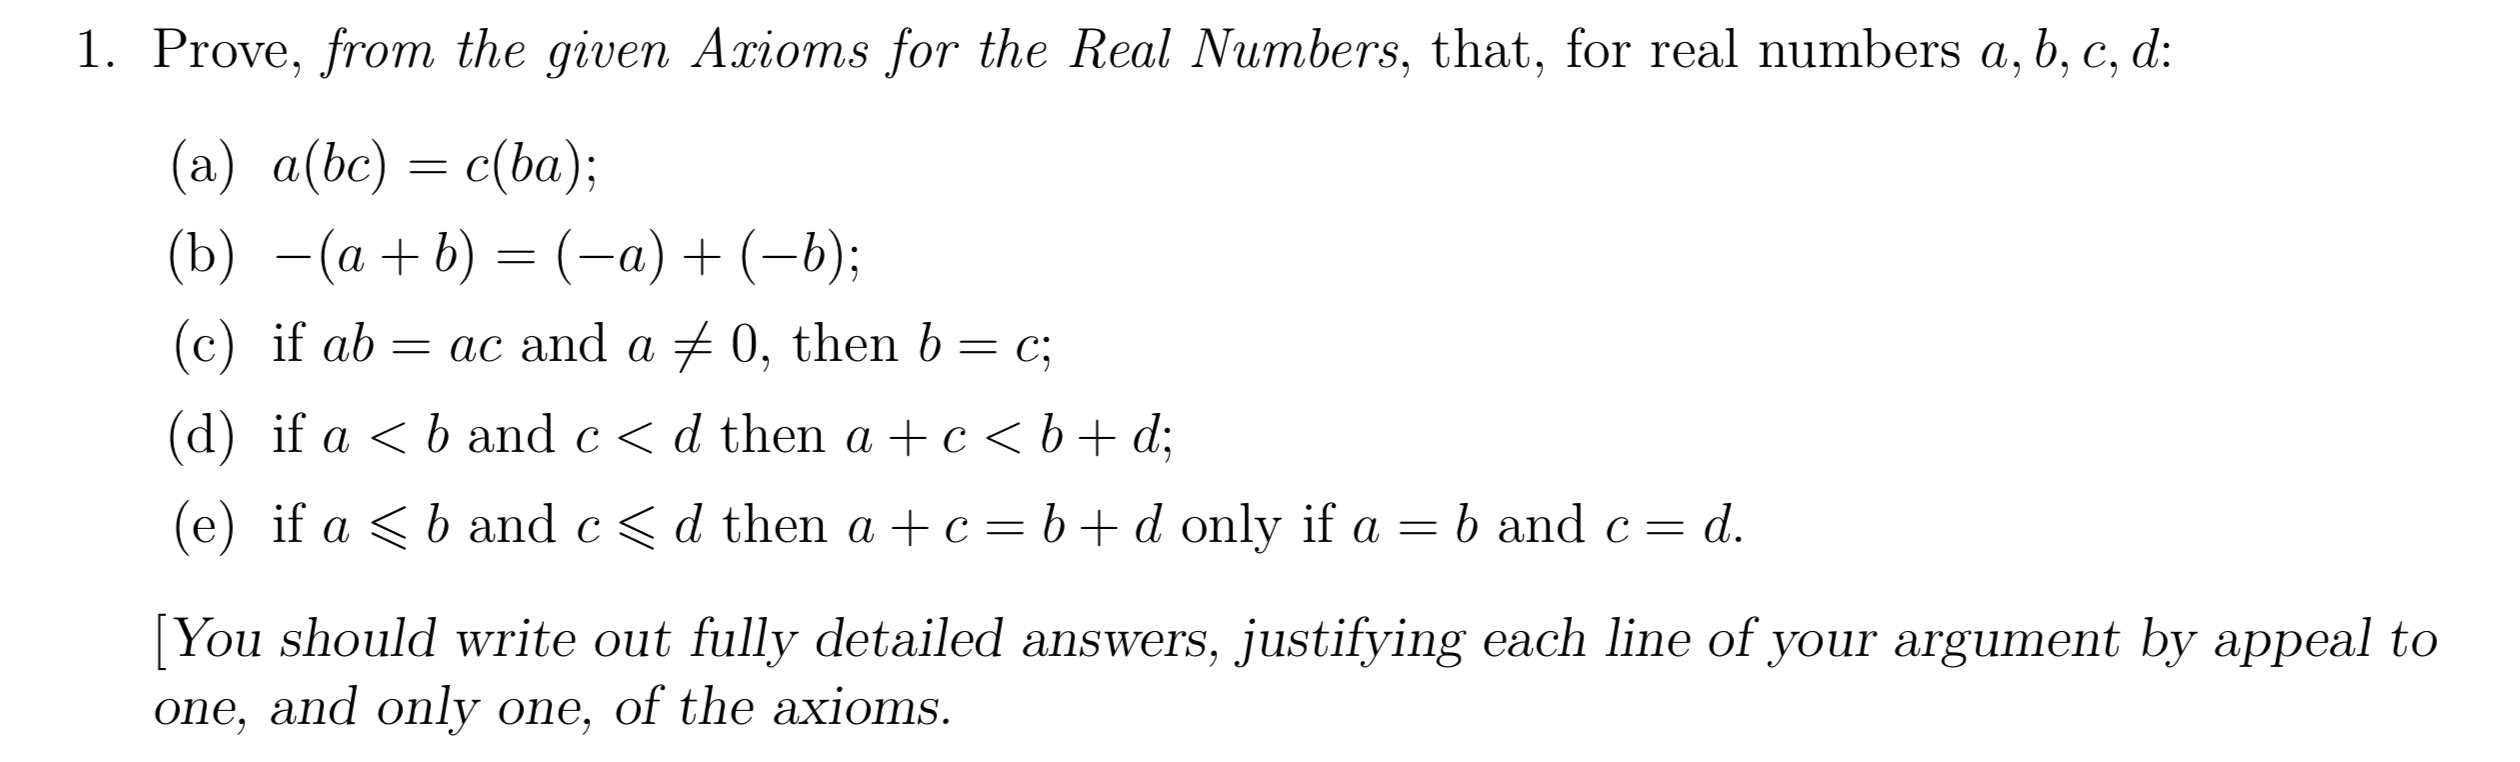
\includegraphics[width=400pt]{img/oxford-M2-analysis-I-1-1.png}
\end{mdframed}

\begin{enumerate}[label=(\alph*)]
\item \begin{theorem*} $a(bc) = c(ba)$\end{theorem*}
  \begin{proof}
    \begin{align*}
      a(bc) &= a(cb)  ~~~~~~~ \text{(M1 commutativity of multiplication)}\\
            &= (ac)b  ~~~~~~~ \text{(M2 associativity of multiplication)}\\
            &= (ca)b  ~~~~~~~ \text{(M1 commutativity of multiplication)}\\
            &= c(ab)  ~~~~~~~ \text{(M2 associativity of multiplication)}\\
            &= c(ba)  ~~~~~~~ \text{(M1 commutativity of multiplication)}
    \end{align*}
  \end{proof}
\newpage
\item
  \begin{theorem*}
    $-(a + b) = (-a) + (-b)$
  \end{theorem*}
  \begin{proof}
    \begin{align*}
      (a + b) + ((-a) + (-b)) &= (a + b) + ((-b) + (-a)) ~~~~~~~ \text{S1 commutativity of sum}\\
                              &=  a + (b + ((-b) + (-a))) ~~~~~~~ \text{S2 associativity of sum}\\
                              &=  a + ((b + (-b)) + (-a)) ~~~~~~~ \text{S2 associativity of sum}\\
                              &=  a + ((-a)) ~~~~~~~ \text{definition of negative}\\
                              &=  0 ~~~~~~~ \text{definition of negative}\\
    \end{align*}
    Therefore $(-a) + (-b)$ is an additive inverse of $a + b$, as claimed. The additive inverse is
    unique by definition.
  \end{proof}
\end{enumerate}

\newpage
\subsection{}
\begin{mdframed}
  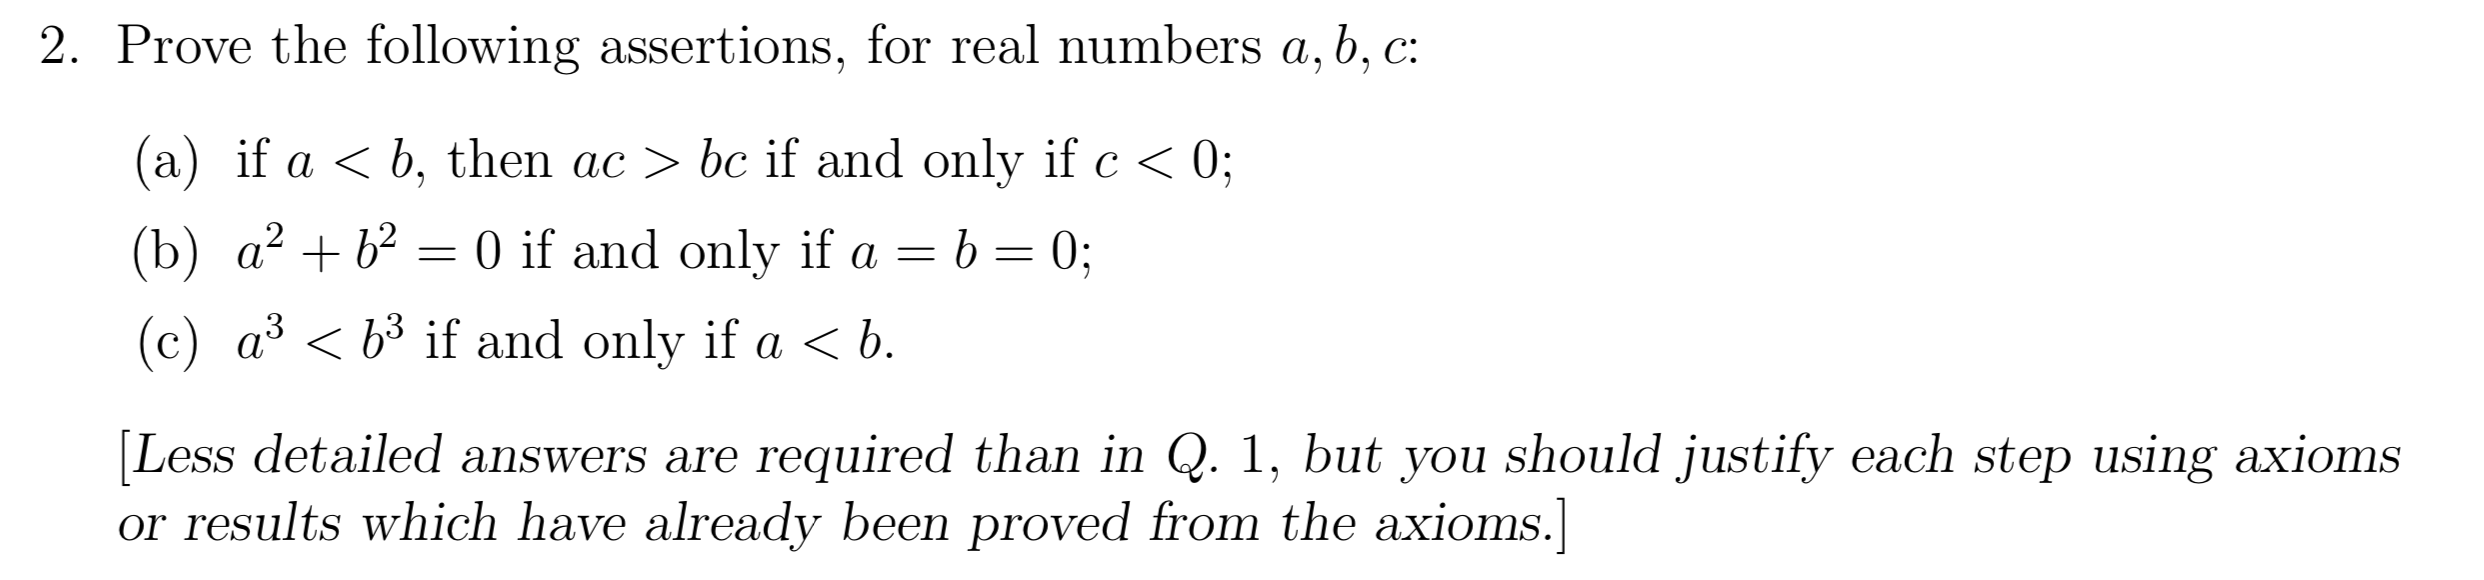
\includegraphics[width=400pt]{img/oxford-prelims-M2-analysis-I-sheet-1-2.png}
\end{mdframed}

\begin{enumerate}[label=(\alph*)]
\item
  \begin{theorem*}
    If $a < b$ then $ac > bc$ iff $c < 0$.
  \end{theorem*}
  \begin{intuition*}
    Multiplication by a scalar flips orientation iff the scalar is negative.
  \end{intuition*}
  \begin{proof}~\\
    \red{TODO} Prove carefully being explicit about which axioms are used.\\
    Let $\P$ be the strictly positive reals. We have $a < b$, i.e. $b - a \in \P$.\\
    $\implies$:\\
    We have $ac > bc$ i.e. $ac - bc \in \P$.

    Therefore
    \begin{align*}
      (a - b)c &\in \P\\
      (b - a)(-c) &\in \P\\
      \frac{1}{b-a}(b - a)(-c) &\in \P\\
      (-c) &\in \P
    \end{align*}

    $\impliedby$:\\
    We have $c < 0$, i.e. $-c \in \P$. Therefore $(-c)(b - a) \in \P$ (by {\bf P2}). Therefore
    $ac - bc \in \P$, i.e. $ac > bc$.
  \end{proof}
\end{enumerate}~\\

\newpage
\subsection{}
\begin{mdframed}
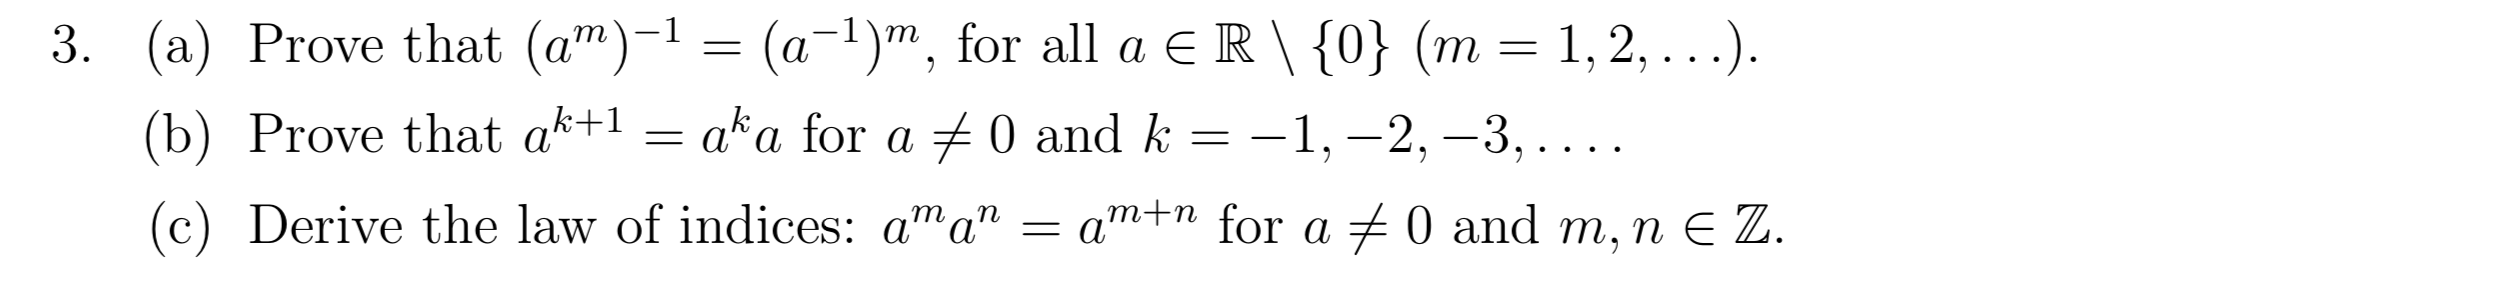
\includegraphics[width=400pt]{img/oxford-prelims-M2-analysis-I-sheet-1-3.png}
\end{mdframed}
\newpage
\subsection{}
\begin{mdframed}
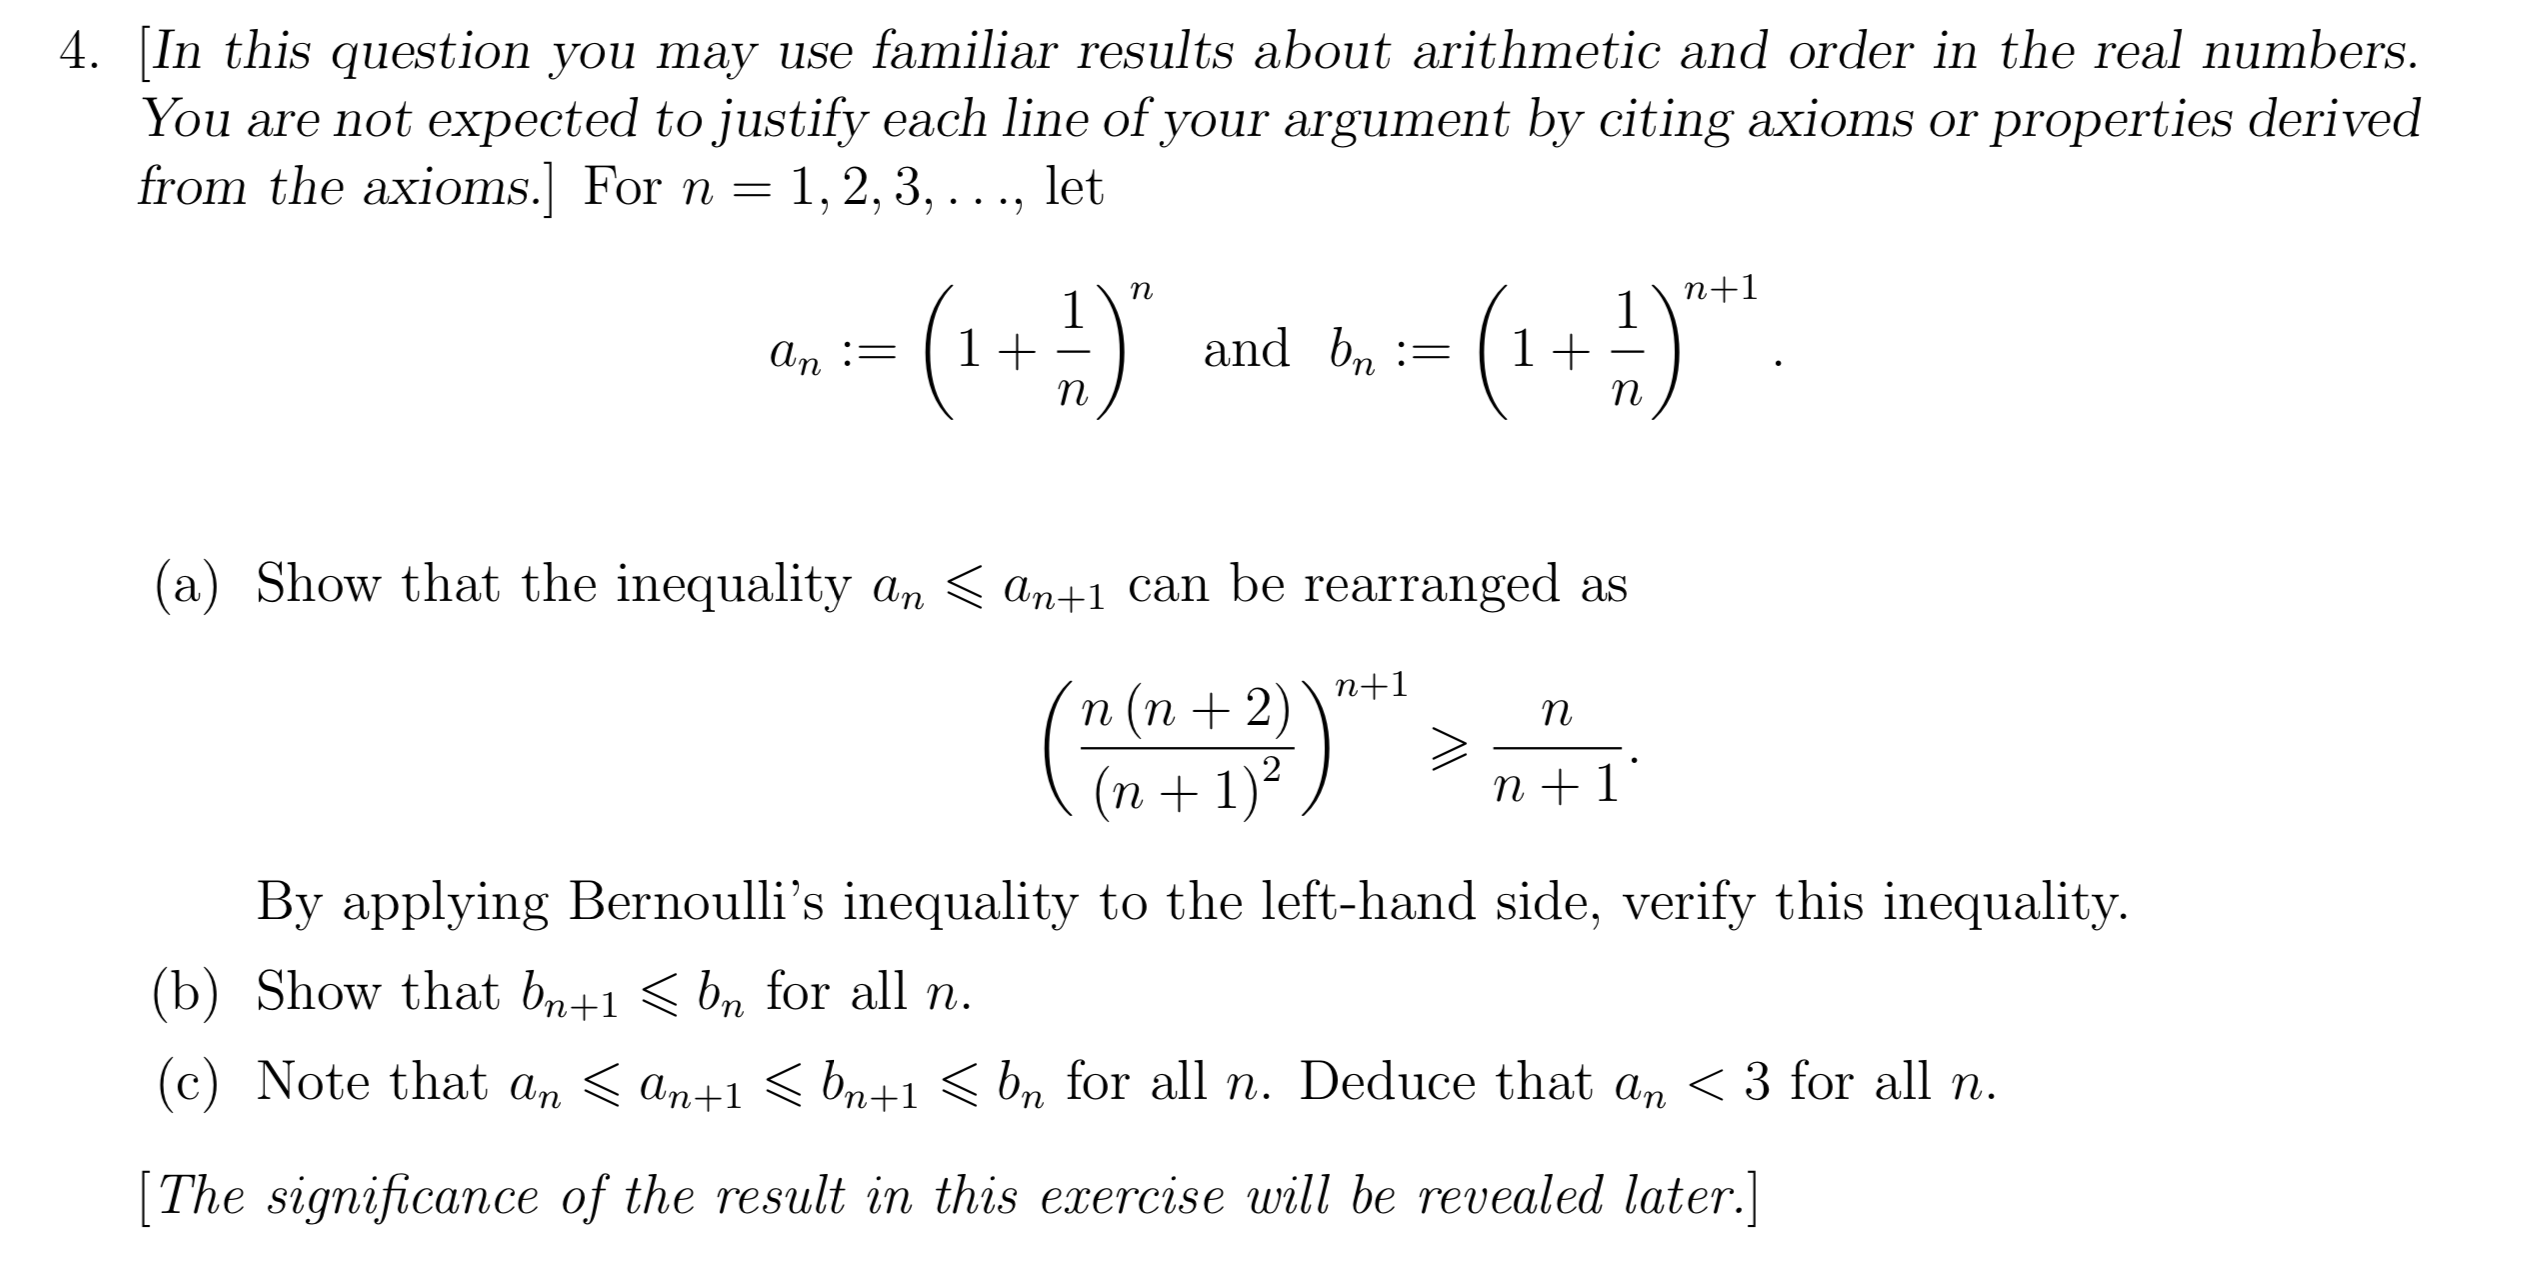
\includegraphics[width=400pt]{img/oxford-prelims-M2-analysis-I-sheet-1-4.png}
\end{mdframed}

\newpage
\subsection{}
\begin{mdframed}
  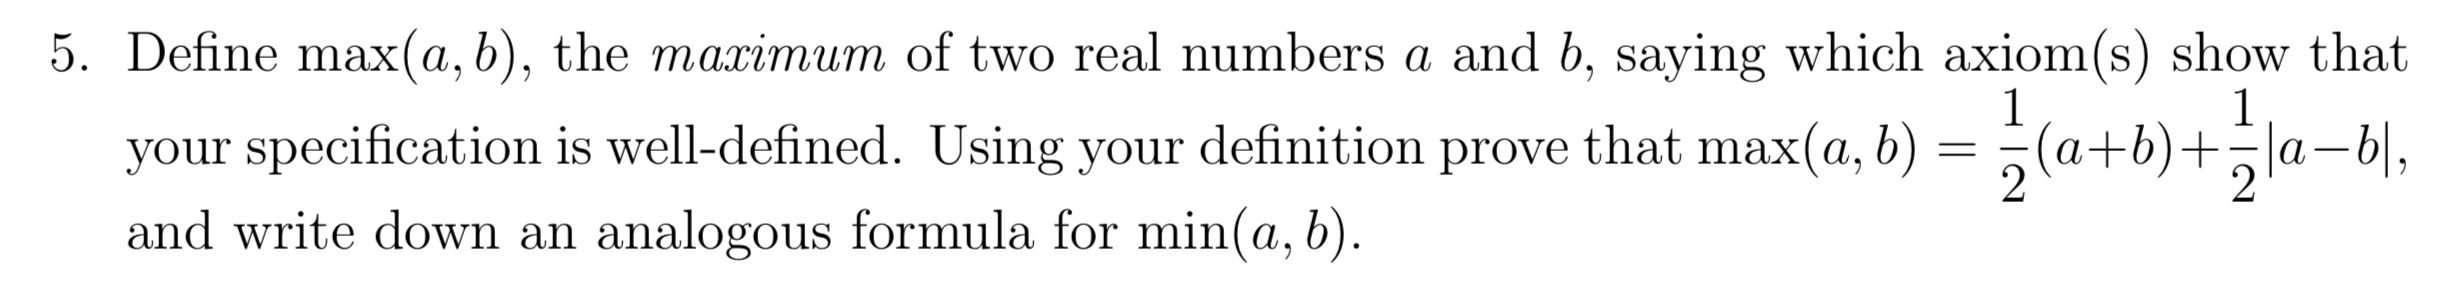
\includegraphics[width=400pt]{img/oxford-M2-analysis-I-1-5.png}
\end{mdframed}

\begin{definition*}
  Let $a, b \in \R$ with $a \neq b$.
  \begin{align*}
    \max(a, b) =
    \begin{cases}
      b ~~~~~~~&\text{if $a < b$}\\
      a ~~~~~~~&\text{if $b \leq a$}.
    \end{cases}
  \end{align*}
  This is well-defined by trichotomy of the order relation ($\max(a, b)$ has a unique value for
  alll $a, b \in \R$ since either $a < b$ or $a = b$ or $a > b$).
\end{definition*}

\begin{theorem*}
  \begin{align*}
    \max(a, b) = \frac{1}{2}(a + b) + \frac{1}{2}|a - b|.
  \end{align*}
\end{theorem*}

\begin{proof}
  Suppose $a = b$. Then
  \begin{align*}
    \frac{1}{2}(a + b) + \frac{1}{2}|a - b|
    = \frac{1}{2}\cdot 2a + \frac{1}{2}\cdot 0
    = a
    = \max(a, b).
  \end{align*}
  Since $(a + b) = (b + a)$ and $|a - b| = |b - a|$, we need only consider $a < b$ as the remaining
  alternative. Then $|a - b| = b - a$ and
  \begin{align*}
    \frac{1}{2}(a + b) + \frac{1}{2}|a - b|
    = \frac{1}{2}(a + b) + \frac{1}{2}(b - a)
    = b
    = \max(a, b).
  \end{align*}
\end{proof}

\newpage
\section{Sheet 2}

\newpage
\subsection{}
\begin{mdframed}
  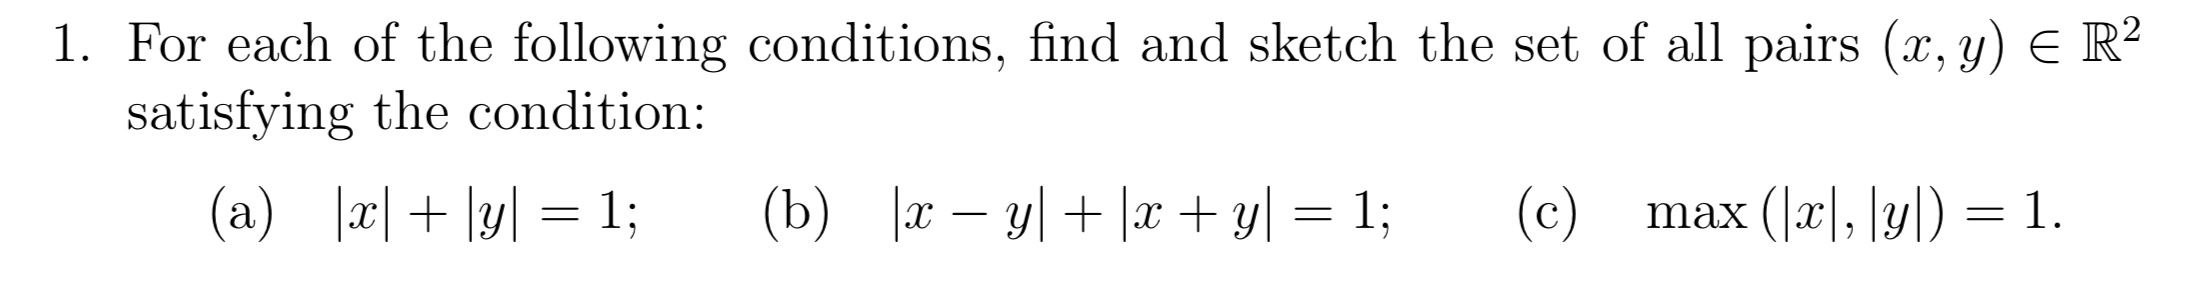
\includegraphics[width=400pt]{img/oxford-M2-analysis-I-2-1.png}
\end{mdframed}

\newpage
\subsection{}
\begin{mdframed}
  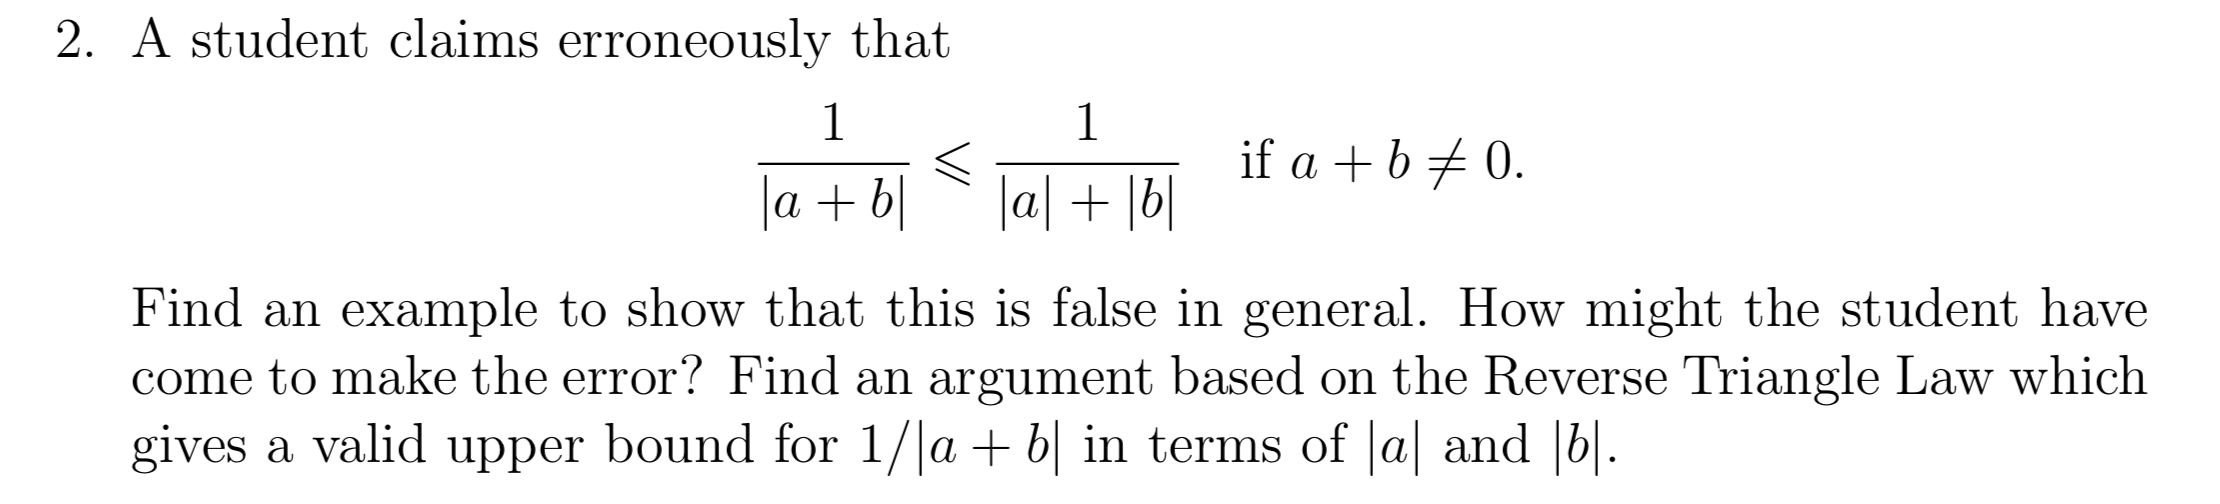
\includegraphics[width=400pt]{img/oxford-M2-analysis-I-2-2.png}
\end{mdframed}

\newpage
\subsection{(COMPLETE)}
\begin{mdframed}
  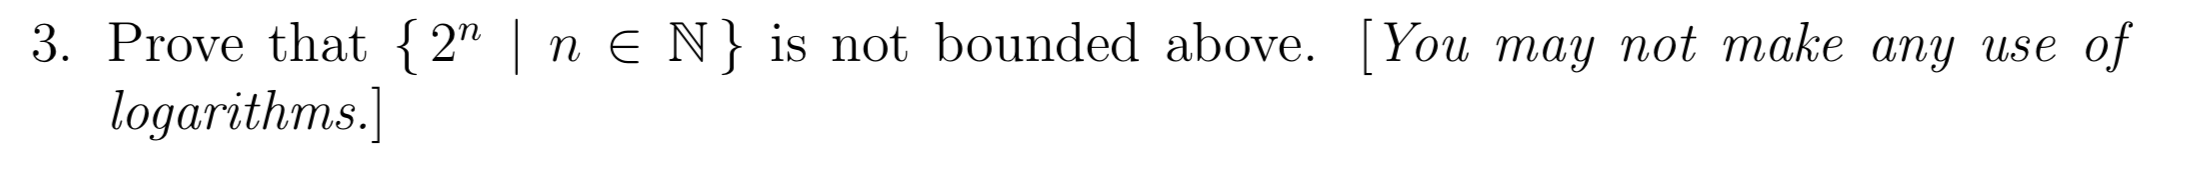
\includegraphics[width=400pt]{img/oxford-M2-analysis-I-2-3.png}
\end{mdframed}

\begin{proof}
  Let $S = \{2^n ~|~ n \in \N\}$ and suppose an upper bound for $S$ exists.

  Then $\sup S$ exists by completeness of the reals.

  By the Approximation Property there exists $2^k \in S$ such that
  \begin{align*}
    \sup S - \frac{1}{2} < 2^k \leq \sup S.
  \end{align*}
  Note that $k+1 \in \N$ therefore $2^{k+1} = 2^k + 2^k \in S$. Therefore
  \begin{align*}
    \sup S - \frac{1}{2} + 2^k &< 2^{k+1} \leq \sup S\\
    \sup S &\leq \sup S + \frac{1}{2} - 2^k < \sup S,
  \end{align*}
  a contradiction. Therefore no upper bound for $S$ exists.
\end{proof}

\newpage
\subsection{(COMPLETE)}
\begin{mdframed}
  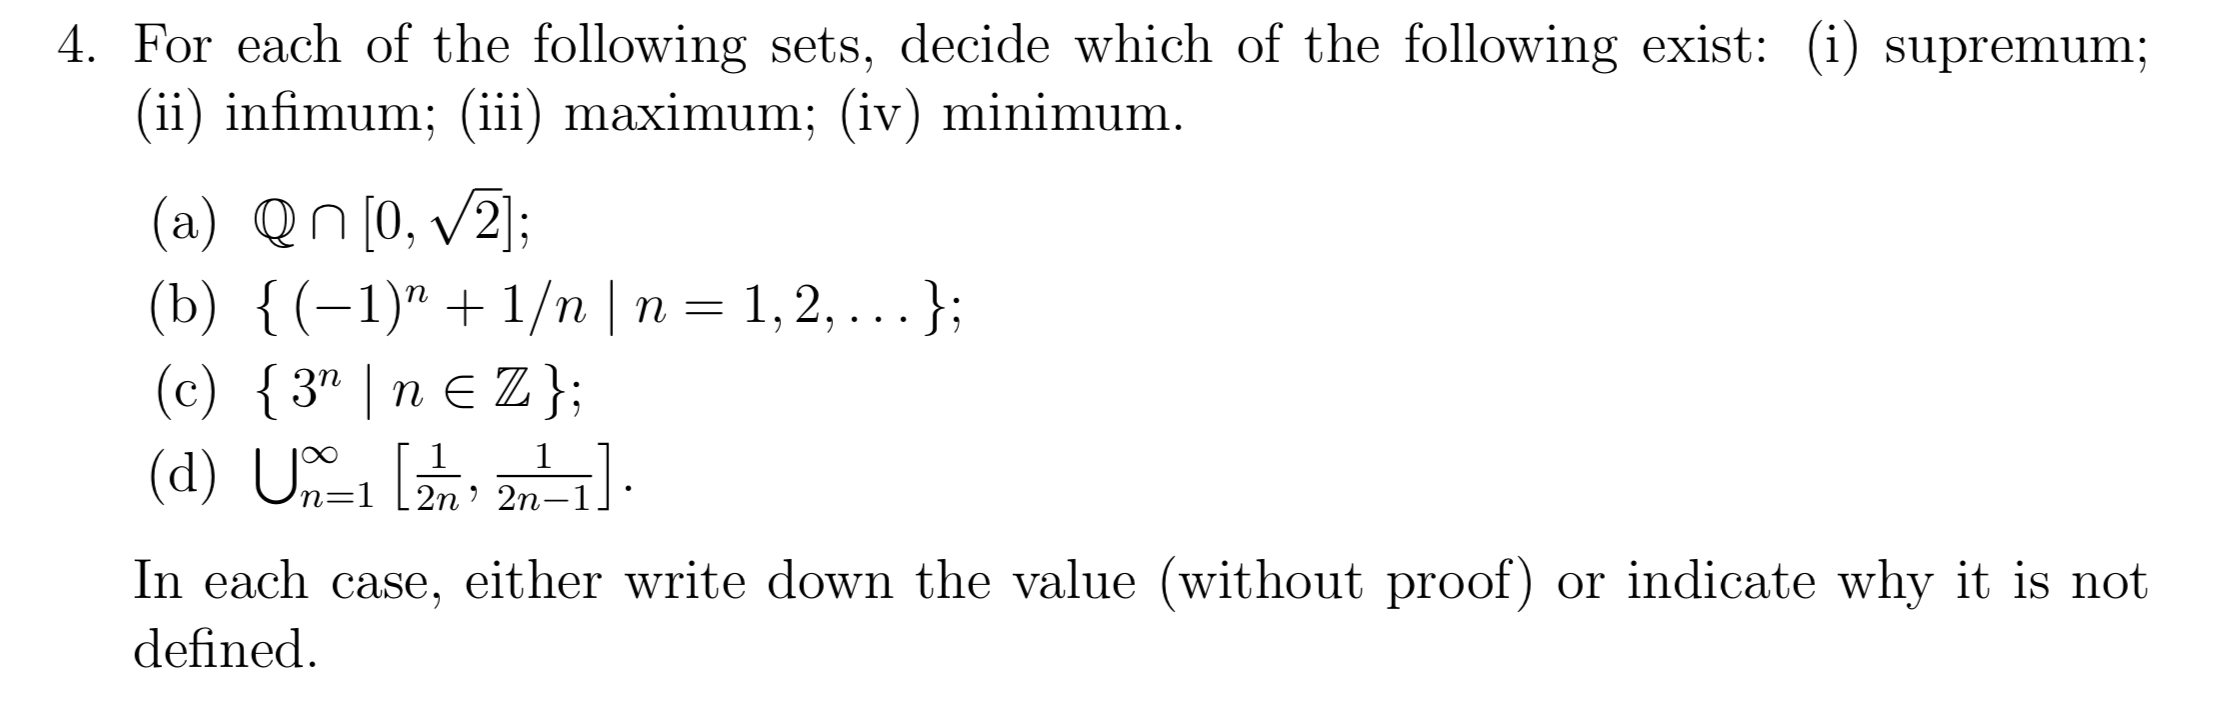
\includegraphics[width=400pt]{img/oxford-M2-analysis-I-2-4.png}
\end{mdframed}
\begin{enumerate}
\item $S = \Q \cap [0, \sqrt 2]$
  \begin{align*}
    \sup S &= \sqrt 2\\
    \max S &= \sqrt 2\\
    \min S &= 0\\
    \inf S &= 0
  \end{align*}
\item $S = \{(-1)^n + 1/n ~|~ n=1,2,\ldots\}$
  \begin{align*}
    \sup S &= 3/2\\
    \max S &= 3/2\\
    \min S ~&\text{does not exist since $\inf S \not\in S$}\\
    \inf S &= -1
  \end{align*}
\item $S = \{3^n ~|~ n \in \Z\}$
  \begin{align*}
    \sup S ~&\text{does not exist, $S$ has no upper bound}\\
    \max S ~&\text{does not exist, $S$ has no upper bound}\\
    \min S ~&\text{does not exist, $S$ has no lower bound}\\
    \inf S &= 0
  \end{align*}
\item $S = \cup_{n=1}^\infty [\frac{1}{2n}, \frac{1}{2n - 1}]$
  \begin{align*}
    \sup S ~&= 1\\
    \max S ~&= 1\\
    \min S ~&\text{does not exist, $S$ has no lower bound}\\
    \inf S ~&=0
  \end{align*}
\end{enumerate}

\newpage
\subsection{(COMPLETE)}
\begin{mdframed}
  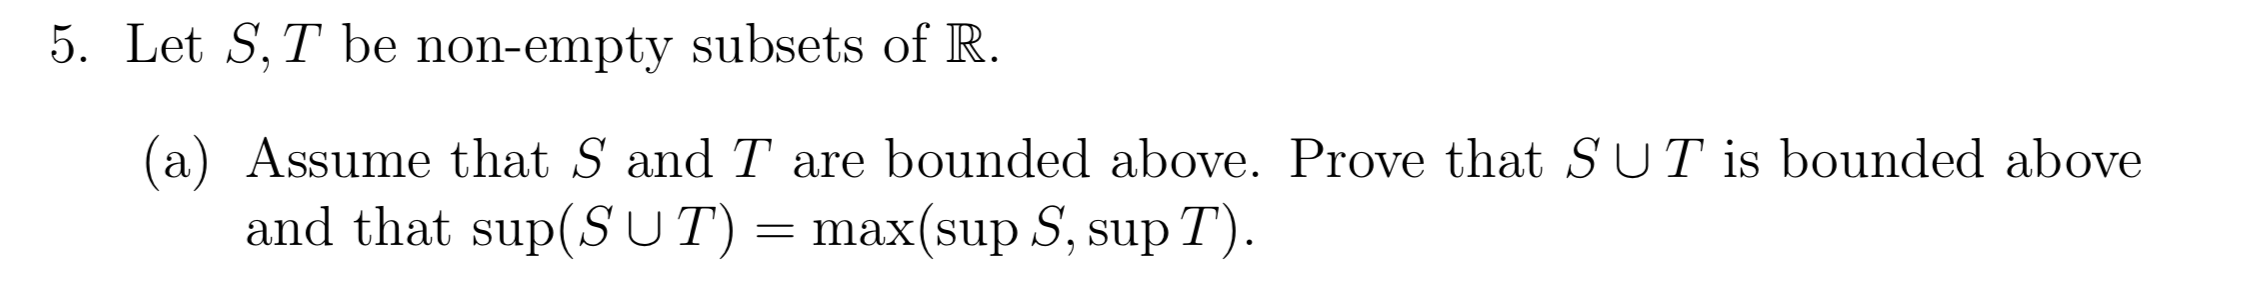
\includegraphics[width=400pt]{img/oxford-M2-analysis-I-2-5-a.png}
\end{mdframed}

\begin{proof}
  Let $S, T \subset \R$ with $S, T \neq \emptyset$. Assume that $S$ and $T$ are bounded
  above. Then $\sup S$ and $\sup T$ exist. Let $b = \max(\sup S, \sup T)$.

  Then $b \geq s$ for all $s \in S$ and $b \geq t$ for all $t \in T$. Therefore $b$ is an upper
  bound for $S \cup T$.

  Suppose there exists $a < b$ such that $a$ is an upper bound of $S \cup T$. Then either
  $a < \sup S$ or $a < \sup T$. Without loss of generality, suppose $a < \sup S$. Then $a$ is not
  an upper bound of $S$. Therefore there exists $s \in S$ such that $s > a$. But
  $s \in S \cup T$, therefore $a$ is not an upper bound of $S \cup T$, a contradiction.
\end{proof}

\begin{mdframed}
  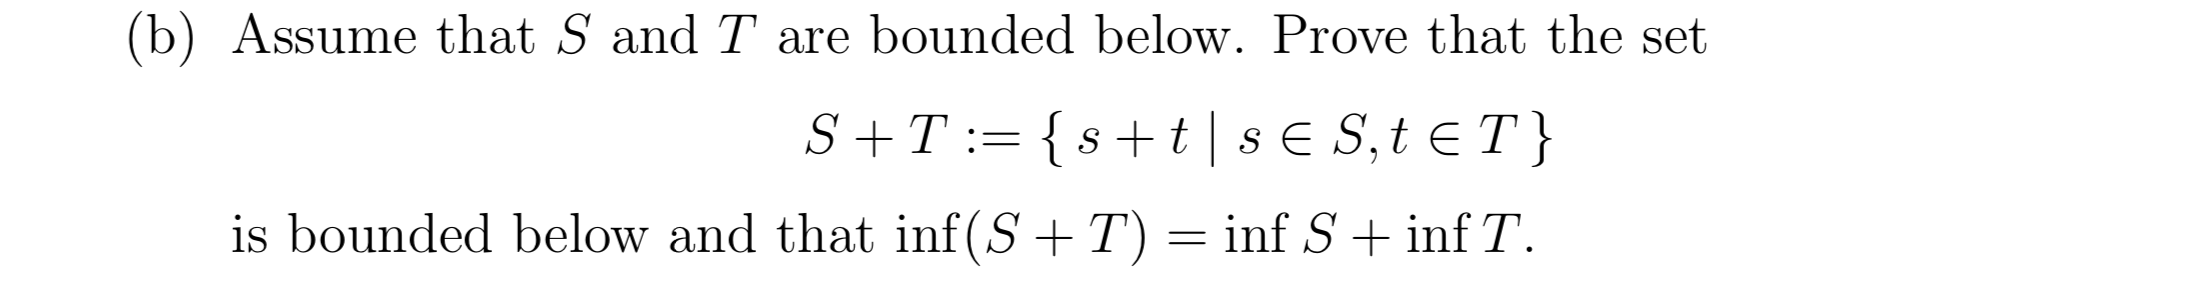
\includegraphics[width=400pt]{img/oxford-M2-analysis-I-2-5-b.png}
\end{mdframed}

\begin{proof}
  Let $S, T \subset \R$ with $S, T \neq \emptyset$. Assume that $S$ and $T$ are bounded
  below. Then $\inf S$ and $\inf T$ exist. Define
  \begin{align*}
    S + T := \{s + t ~|~ s \in S, t \in T\}.
  \end{align*}
  Let $a = \inf S + \inf T$.

  We claim that $a$ is a lower bound for $S + T$, i.e. $u \geq a$ for all $u \in S + T$.

  Let $u \in S + T$. Then $u = s + t$ for some $s \in S, t \in T$. Therefore
  $$u = (\inf S + v) + (\inf T + w) = a + (v + w) \geq a$$ for some $v, w \geq 0$. Therefore $a$ is
  a lower bound for $S + T$ as claimed.

  We further claim that $a = \inf S + T$.

  Suppose for a contradiction that there exists $b > a$ such that $b$ is a lower bound for
  $S + T$. Then $$b = a + v + w = (\inf S + v) + (\inf T + w)$$ for some $v, w > 0$. Fix
  $0 < \delta < \min(v, w)$. By {\bf 4.9} (Approximation Property of the supremum/infimum) there
  exist $s \in S$ and $t \in T$ such that $\inf S \leq s < \inf S + \delta$ and
  $\inf T \leq t < \inf T + \delta$. But then $s + t \in S + T$ and $s + t < b$, so $b$ is not a
  lower bound for $S + T$, a contradiction. Therefore $a = \inf S + T$ as claimed.
\end{proof}

\newpage
\subsection{}
\begin{mdframed}
  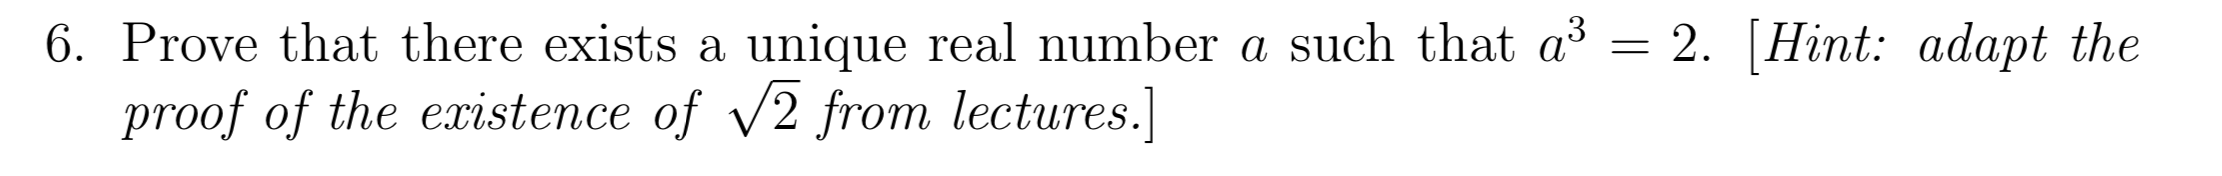
\includegraphics[width=400pt]{img/oxford-M2-analysis-I-2-6.png}
\end{mdframed}

\begin{proof}
  Let $S = \{x \in \R ~|~ x^3 < 2\}$. Since $S$ is bounded above, $\sup S$ exists. Let
  $a = \sup S$. By trichotomy it suffices to show that $a^3 < 2$ and $a^3 > 2$ lead to
  contradictions.

  First suppose $a^3 < 2$. We seek $h > 0$ such that $(a + h)^3 < 2$ since then $a + h \in S$,
  which would contradict the definition $a := \sup S$. Note that
  \begin{align*}
    (a + h)^3 &= a^3 + 3a^2h + 3ah^2 + h^3 - 2\\
              &< a^3 + 7a^2h - 2 ~~~~~~~~~~~~~~~~~~~~~~~~\text{if $h < a$}\\
              &< 0              ~~~~~~~~~~~~~~~~~~~~~~~~~~~~~~~~~~~~~~~~~\text{if $h < \frac{2 - a^3}{7a^2}$},
  \end{align*}
  therefore if we take $h < \min\(a, \frac{2 - a^3}{7a^2}\)$ then we have the desired
  contradiction.

  Alternatively suppose that $a^3 > 2$. By the Approximation Property for all $0 < h < a$ we can
  find $s \in S$ such that $a - h < s$, therefore $(a - h)^3 < s^3$. We seek an $h$ for which
  $(a - h)^3 > 2$ since then we would have $s^3 > 2$ which would contradict the definition of
  $S$. Note that
  \begin{align*}
    (a - h)^3 - 2 &= a^3 - 3a^2h + 3ah^2 - h^3 - 2\\
                  &> 0 ~~~~~~~~~~~~~~~~~~~~~~~~~~~~~~~~~~~~~~~~~\text{if $3ah^2 > 3a^2h + h^3$}.
  \end{align*}
  So we require $3ah > 3a^2 + h^2 \iff 3a^2 - 3ah + h^2 < 0$.

  \red{Incomplete}
\end{proof}

\newpage
\subsection{}
\begin{mdframed}
  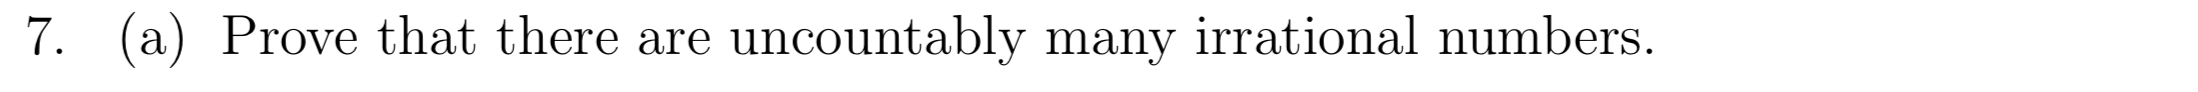
\includegraphics[width=400pt]{img/oxford-M2-analysis-I-2-7-a.png}
\end{mdframed}
\begin{definition*}[Countable]
  A set $S$ is countable if $S \preceq N$. I.e. there exists an injection $f:S \to \N$.
\end{definition*}
\begin{definition*}[Uncountable]
  A set $S$ is uncountable if it is not countable.
\end{definition*}
\begin{definition*}[Injection]
  A function $A \to B$ is an injection if $f(a_1) = f(a_2) \implies a_1 = a_2$.
\end{definition*}
\begin{proof}
  Suppose for a contradiction that $\R \setminus \Q$ is countable. Then an injection
  $f:\R \setminus \Q \to \N$ exists. Since $\Q$ is countable, an injection $g:\Q \to \N$
  exists. Consider the function $h:\R \to \N$ defined by
  \begin{align*}
    h(x) =
    \begin{cases}
      2f(x) &x \in \R \setminus \Q\\
      2g(x) + 1 &x \in \Q.
    \end{cases}
  \end{align*}
  We claim that $h:\R \to \N$ is an injection. Note that
  \begin{enumerate}[label=(\roman*)]
  \item $h(\R\setminus\Q) \cap h(\Q) = \emptyset$
  \item The $\R \to \R$ functions defined by $x \mapsto 2x$ and $x \mapsto 2x + 1$ are both
    injections.
  \item The composition of two injections is an injection.
  \end{enumerate}
  Suppose $h(x_1) = h(x_2)$. Then either $x_1, x_2 \in \Q$ or $x_1, x_2 \in \R\setminus\Q$ by
  (i). In both cases we have $x_1 = x_2$ by (ii) and (iii). Therefore $h:\R \to \N$ is an
  injection, hence $\R$ is countable.

  But $\R$ is not countable, so we have a contradiction. Therefore no such injection $f$ exists,
  i.e. $\R\setminus\Q$ is uncountable.
\end{proof}

\begin{lemma*}
  Let $a, b$ be real numbers with $a < b$. Let $\delta \in \R$ with $0 < \delta < b - a$. Then
  there exists $m \in \N$ such that $m\delta \in (a, b)$.
\end{lemma*}

\begin{proof}
  Let $m \in \N$, $\delta \in \R$ with $0 < \delta < b - a$, and define
  $S = \{m\delta ~|~ m\delta < b\}$. Note that $\delta \in S$. Therefore $S$ is non-empty, bounded
  above, and finite, hence $\max S$ exists.

  Let $M\delta = \max S$. We have $M\delta < b$. Suppose for a contradiction that $M\delta \leq
  a$. Recall that $\delta < b - a$. Summing these inequalities gives $(M + 1)\delta < b$. But then
  $M\delta \neq \max S$ since $(M + 1)\delta > M\delta$ and $(M + 1)\delta \in S$. This is a
  contradiction, therefore $M\delta \in (a, b)$.
\end{proof}

\begin{mdframed}
  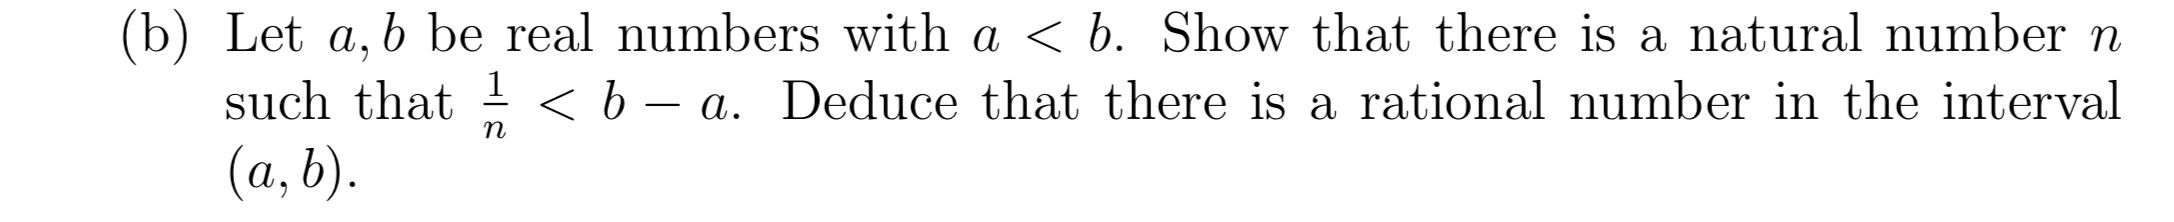
\includegraphics[width=400pt]{img/oxford-M2-analysis-I-2-7-b.png}
\end{mdframed}

\begin{proof}
  Let $a, b \in \R$ with $a < b$. Then $b - a > 0$. Since $\N$ is not bounded above (Archimedean
  property) there exists $n \in \N$ such that $n > 1/(b - a)$, therefore $1/n < b - a$. Therefore,
  by the lemma with $\delta = 1/n$, there exists $m \in \N$ such that $m/n \in (a, b) \cap \Q$.
\end{proof}

\begin{mdframed}
  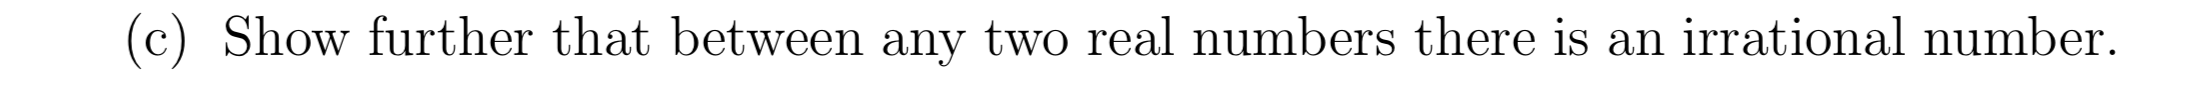
\includegraphics[width=400pt]{img/oxford-M2-analysis-I-2-7-c.png}
\end{mdframed}

\begin{proof}
  Let $a, b \in \R$ with $a < b$. By the Archimedean property of $\N$, there exists $n \in \N$ be
  such that $1/n < (b - a)/\pi$, therefore $\pi/n < (b - a)$. Therefore, by the lemma with
  $\delta = \pi/n$, there exists $m \in \N$ such that $m\pi/n \in (a, b) \cap (\R\setminus\Q)$.
\end{proof}
\newpage
\subsection{}
\begin{lemma*}
  The set of polynomials of degree $n$ with integer coefficients is countable.
\end{lemma*}
\begin{proof}
  Let $\{\alpha_1, \alpha_2, \ldots\}$ be the positive prime numbers and let
  $$P_n := \Big\{\sum_{i=0}^n a_iz^i ~|~ a_0, \ldots, a_n \in \Z, a_n \neq 0\Big\}$$ be the set of
  polynomials with integer coefficients of degree $n$. Note that
  $|P_n| = \big|\(\Z\setminus\{0\}\) \times \Z^{n-1}\big|$ and that
  $f:\(\Z\setminus\{0\}\) \times \Z^{n-1} \to \N$ given by
  \begin{align*}
    f(a_0, a_1, \ldots, a_n) = \prod_{i=0}^n\alpha_i^{a_i}\
  \end{align*}
  is a bijection by uniqueness of prime factorization of the natural numbers. Therefore $P_n$ is
  countable.
\end{proof}

\begin{mdframed}
  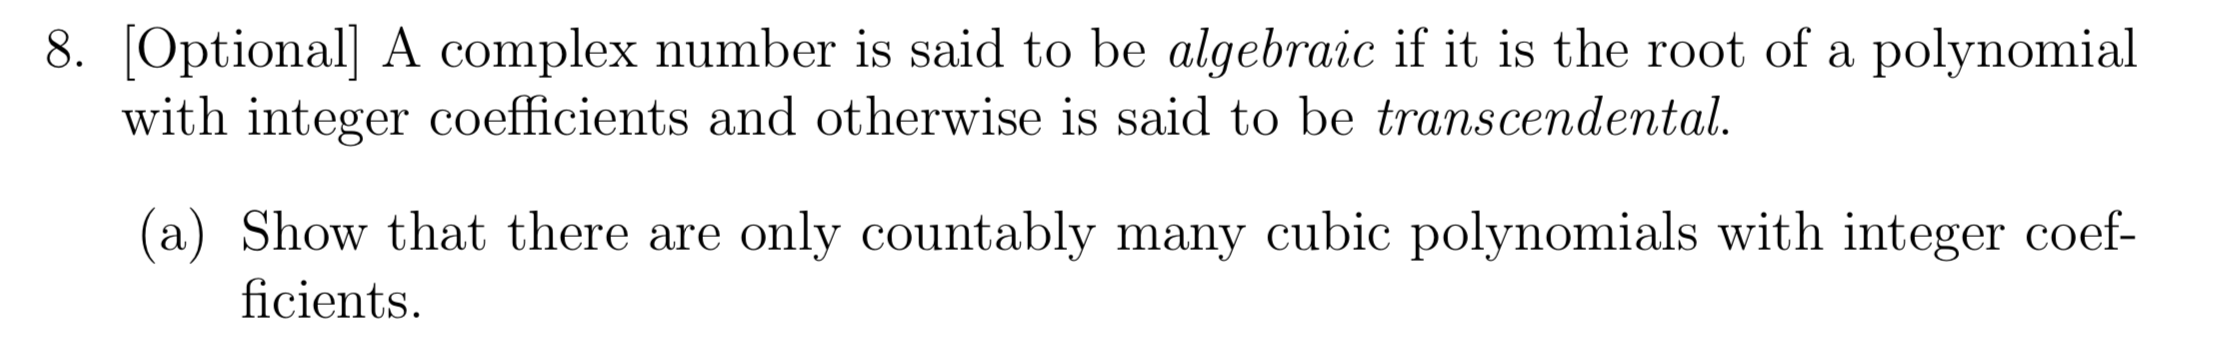
\includegraphics[width=400pt]{img/oxford-M2-analysis-I-2-8-a.png}
\end{mdframed}

\begin{proof}
  This follows from the lemma with $n=3$.
\end{proof}

\begin{lemma*}[Countable union of countable sets is countable]~\\
  Let $I \subseteq \N$ and let $S_i$ be a countable set for all $i \in I$. Then
  $\bigcup_{i\in I}S_i$ is countable.
\end{lemma*}
\begin{proof}
  Let $s_{ij}$ be the $j$-th element of $S_i$. The $f:\bigcup_{i\in I}S_i \to \N$ given by
  \begin{align*}
    f(s_{ij}) = 2^i3^j
  \end{align*}
  is a bijection, proving that $\bigcup_{i\in I}S_i$ is countable.
  \red{But what about repeated elements?}
\end{proof}

\begin{mdframed}
  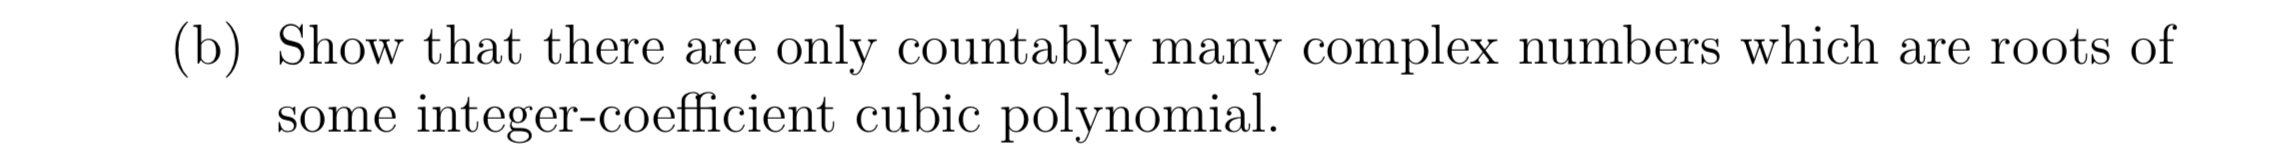
\includegraphics[width=400pt]{img/oxford-M2-analysis-I-2-8-b.png}
\end{mdframed}

\begin{lemma*}
  Let $P_n$ be the set of polynomials with integer coefficients of degree $n$. Then the set of
  complex numbers that are roots of a polynomial in $P_n$ is countable.
\end{lemma*}
\begin{proof}
  Let $P_{n,k}$ be the set of polynomials of degree $n$ that have $k \leq n$ distinct roots. Since
  $P_{n,k} \subseteq P_n$, we have that $P_{n,k}$ is countable. Therefore For each polynomial in
  $P_{n,k}$ order the $k$ distinct roots and label them $1, \ldots, k$. Then $P_{n,k}$ is countable
  since...
\end{proof}

\begin{proof}
  Note that a cubic polynomial has at most 3 distinct roots.

  Let $U$ be the set of complex numbers that are roots of some integer-coefficient cubic
  polynomial. For each such polynomial, assign a distinct label from $\{0, 1, 2\}$ to each of the
  distinct roots. Then the cardinality of $U$ is equal(*) to the cardinality of
  $B := \Z\setminus\{0\} \times \Z^3 \times \{0, 1, 2\}$. The set $B$ is countable since
  $f:T \to \N$ given by $f(a, b, c, d, e) = 2^a3^b5^c7^d11^e$ is an injection. (\red{* How to
    properly deal with the fact that $U$ is smaller than $B$ due to some polynomials having fewer
    than 3 distinct roots?})
\end{proof}

\begin{mdframed}
  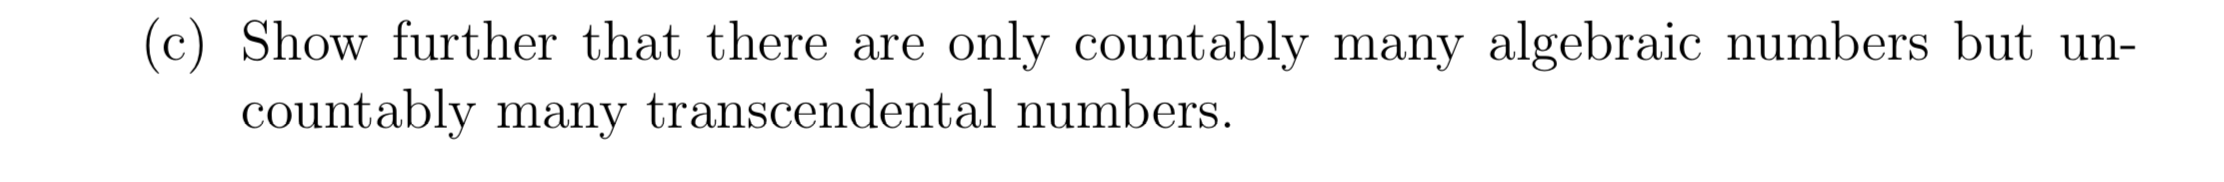
\includegraphics[width=400pt]{img/oxford-M2-analysis-I-2-8-c.png}
\end{mdframed}

\begin{proof}
  Let $A_n$ be the set of complex numbers which are roots of a polynomial of degree $n$.

  Claim: $A_n$ is countable for all $n \in \N$, since there are countably many polynomials of
  degree $n$ and each has a finite number of roots.

  The set of algebraic numbers is $A := \cup_{n\in\N} A_n$. Let $a_{ijk}$ be the $k$-th distinct
  root of the $j$-th polynomial of degree $i$. Then $f:$

  (This differs because whereas previously we were restricted to cubics, now the polynomials can
  be of any degree $n \in \N$.)

  The cardinality of the set of algebraic numbers is \red{Incomplete}.
\end{proof}
\newpage
\section{Sheet 3}

\subsection{}
\begin{mdframed}
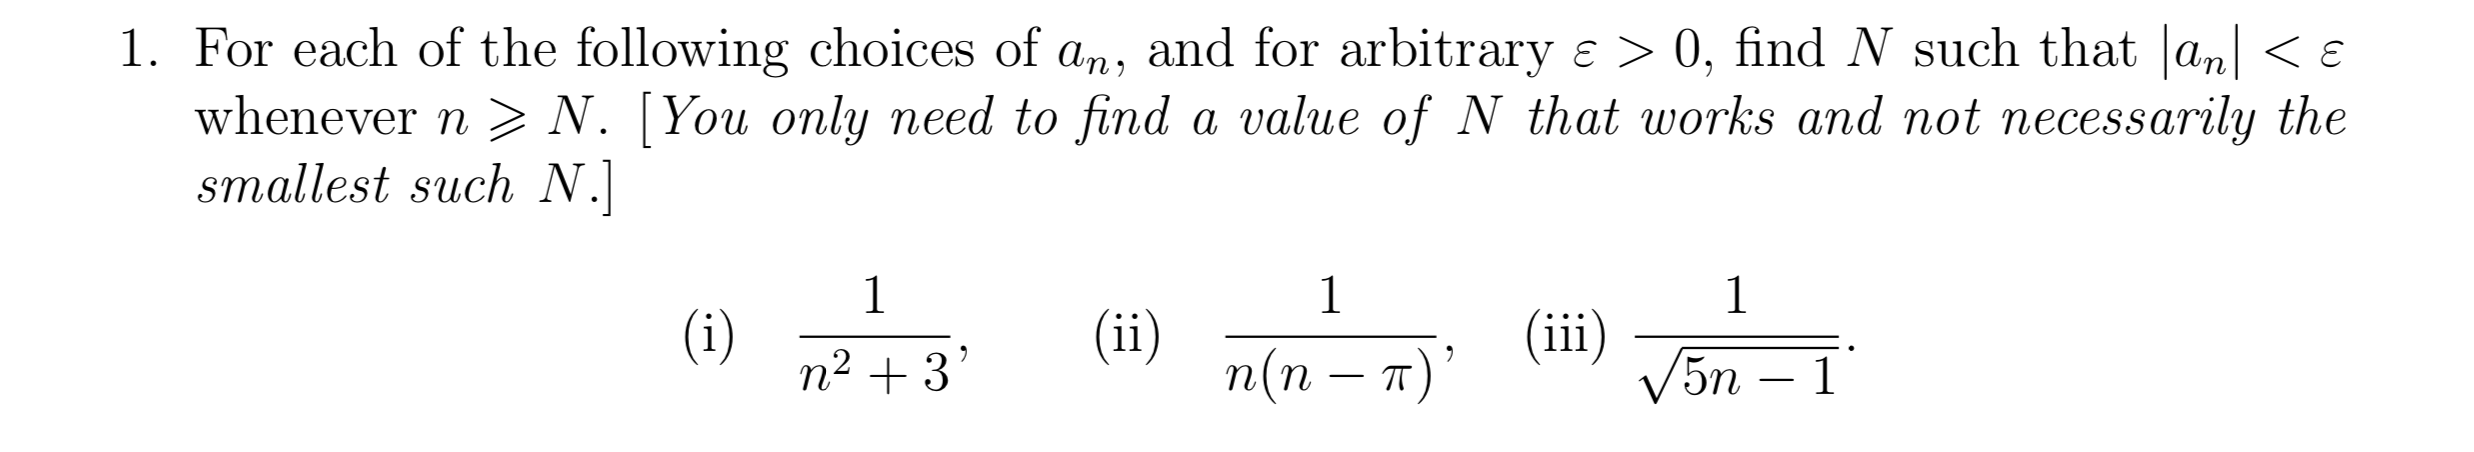
\includegraphics[width=400pt]{img/oxford-M2-analysis-I-3-1.png}
\end{mdframed}

\begin{enumerate}[label=(\roman*)]
\item Take $n = \ceil{\frac{1}{\sqrt{\epsilon}}}$. Then
  $
    |a_n| < \frac{1}{\ceil{\frac{1}{\sqrt{\epsilon}}}^2}
          \leq \frac{1}{\frac{1}{\epsilon}}
          = \epsilon.
  $
  Therefore $N = \ceil{\frac{1}{\sqrt{\epsilon}}}$ works.
\item Note that $|n(n - \pi)| = n|n - \pi| > n$ for $n \geq 4$. Therefore
  \begin{align*}
    |a_n| = \frac{1}{|n(n - \pi)|} &< \frac{1}{n} ~~~~~~~\text{if $n \geq 4$}\\
                                   &< \epsilon    ~~~~~~~\text{if $n > \Bigceil{\frac{1}{\epsilon}}$}.
  \end{align*}
  Therefore $N = \max\(1 + \Bigceil{\frac{1}{\epsilon}}, 4\)$ works.
\item Take $n = \Bigceil{\frac{1}{5\epsilon^2} + \frac{1}{5}}$. Then $|a_n| \leq
  \epsilon$. Therefore $N = \Bigceil{\frac{1}{5\epsilon^2}} + 1$ works.
\end{enumerate}

\newpage
\subsection{}
\begin{mdframed}
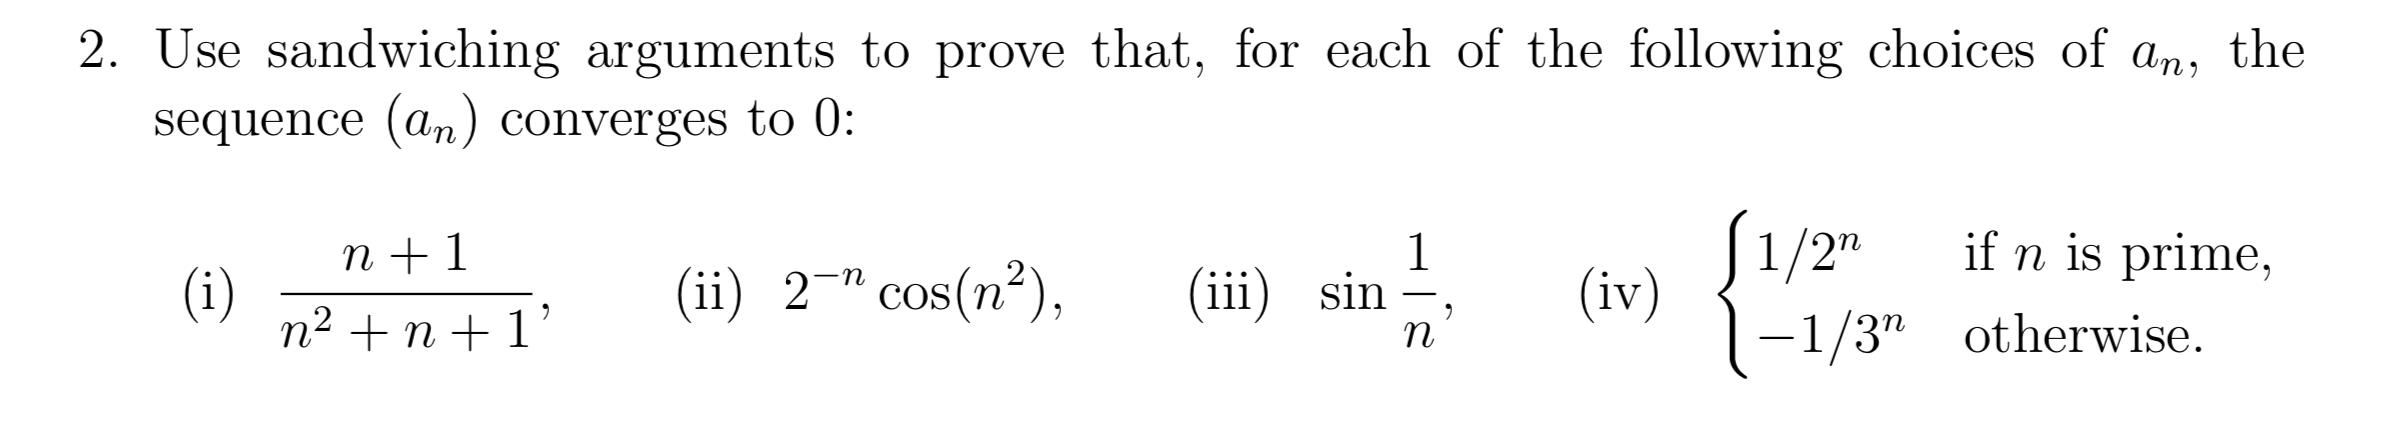
\includegraphics[width=400pt]{img/oxford-M2-analysis-I-3-2.png}
\end{mdframed}

\begin{enumerate}[label=(\roman*)]
\item Note that
  \begin{align*}
    0 < a_n
    = \frac{n + 1}{n^2 + n + 1}
    = \frac{1}{n + 1 + 1/n} + \frac{1}{n^2 + n + 1}
    < \frac{1}{n} + \frac{1}{n^2}.
  \end{align*}
  Therefore $a_n \to 0$, since $\frac{1}{n} + \frac{1}{n^2} \to 0$.
\item Note that $\cos n^2$ is bounded and that $2^{-n} \to 0$. Therefore
  $a_n = 2^{-n}\cos n^2 \to 0$.
\item Note that $0 \leq \sin x \leq x$ for all $0 \leq x \leq \pi$. Therefore
  $0 \leq a_n = \sin \frac{1}{n} \leq \frac{1}{n}$ for all $n \geq 4$. We have $\frac{1}{n} \to 0$,
  therefore $a_n \to 0$ by the Sandwiching Lemma and the Tails Lemma.
\item Note that $-\frac{1}{3^n} \leq a_n \leq \frac{1}{2^n}$. Therefore by $a_n \to 0$ by the
  Sandwiching Lemma since $-\frac{1}{3^n} \to 0$ and $\frac{1}{2^n} \to 0$.
\end{enumerate}

\newpage
\subsection{}
\begin{mdframed}
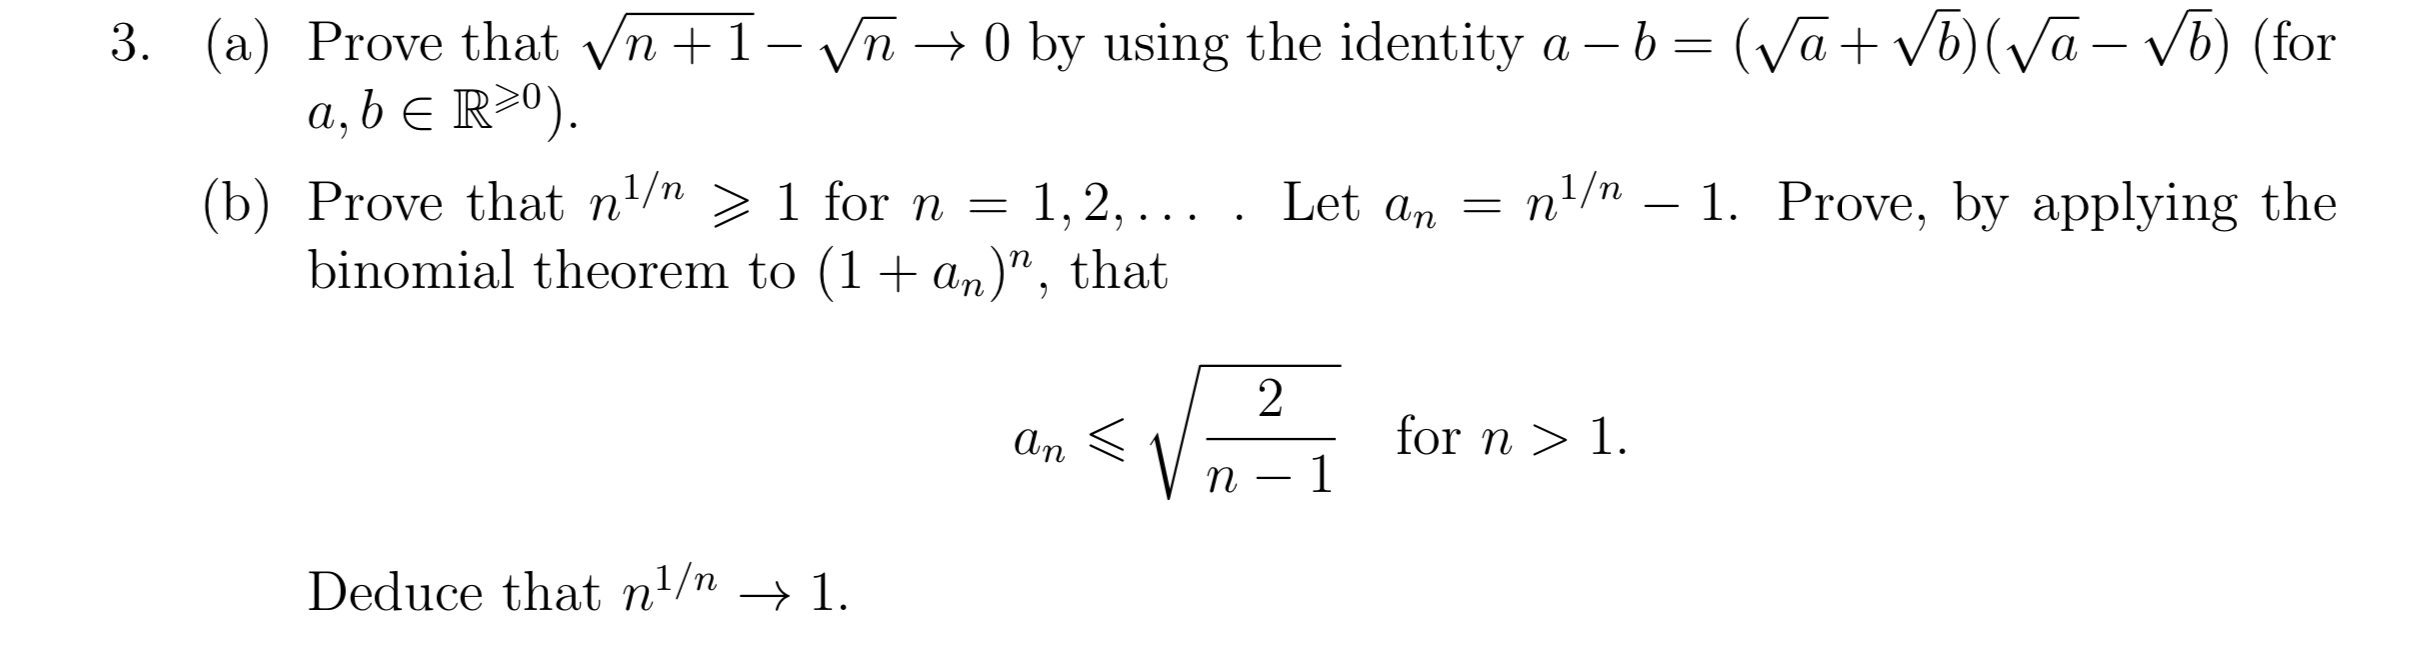
\includegraphics[width=400pt]{img/oxford-M2-analysis-I-3-3.png}
\end{mdframed}

\begin{enumerate}[label=(\alph*)]
\item
  \begin{theorem*}
    $\sqrt{n+1} - \sqrt{n} \to 0$.
  \end{theorem*}

  \begin{proof}
    Note that for $n \geq 1$
    \begin{align*}
      \sqrt{n+1} - \sqrt{n}
      = \frac{n + 1 - n}{\sqrt{n+1} + \sqrt{n}}
      = \frac{1}{\sqrt{n+1}} + \frac{1}{\sqrt{n}}.
    \end{align*}
    Further, note that $\frac{1}{\sqrt{n}} \to 0$ since for all $\epsilon > 0$ if
    $n \geq \ceil{\frac{1}{\epsilon^2}} + 1$ we have $\frac{1}{\sqrt{n}} < \epsilon$.

    Also $0 < \frac{1}{\sqrt{n+1}} < \frac{1}{\sqrt{n}}$ therefore $\frac{1}{\sqrt{n+1}} \to 0$ by
    the Sandwiching Lemma.

    Therefore $\sqrt{n+1} - \sqrt{n} \to 0 + 0 = 0$ by Algebra of Limits.
  \end{proof}
\item
  \begin{theorem*}
    $n^{1/n} \geq 1$ for $n = 1, 2, \ldots$.
  \end{theorem*}
  \begin{proof}
    Suppose there exists $n \in \N$ such that $n^{1/n} < 1$. Let $\alpha = n^{1/n} < 1$. Then
    $\alpha^n \geq 1$ since $\(n^{1/n}\)^n = n \in \N$. But we can prove by induction that
    $\alpha^n < 1$: We have $\alpha^1 < 1$; suppose $\alpha^k < 1$. Then
    $\alpha^{k+1} = \alpha\alpha^k < 1$. Therefore $\alpha^n < 1$ for $n = 1, 2, \ldots$ by
    induction. This contradiction proves that $n^{1/n} \geq 1$ for $n = 1, 2, \ldots$.
  \end{proof}

  \begin{theorem*}
    Let $a_n = n^{1/n} - 1$. Then $a_n \leq \sqrt{\frac{2}{n - 1}}$ for $n > 1$.
  \end{theorem*}
  \begin{proof}
    Note that $n = (1 + a_n)^n > 1 + na_n + \frac{n(n-1)}{2}a_n^2$, therefore for $n > 1$ we have
    $\frac{n(n-1)}{2}a_n^2 < n$, therefore $a_n < \sqrt{\frac{2}{n - 1}}$.
  \end{proof}
  \begin{theorem*}
    $n^{1/n} \to 1$.
  \end{theorem*}
  \begin{proof}
    Fix $\epsilon > 0$. Note that if $n = \ceil{\frac{1}{2\epsilon^2}} + 1$ then
    $0 < \sqrt{\frac{2}{n - 1}} \leq \epsilon$. Let $N = \ceil{\frac{1}{2\epsilon^2}} + 2$. Then
    $|a_n - 0| < \epsilon$ for all $n \geq N$. Therefore $a_n \to 0$ and $n^\frac{1}{n} \to 1$.
  \end{proof}
\end{enumerate}



\newpage
\subsection{}
\begin{enumerate}[label=(\alph*)]
\item\hspace{0pt}
  \begin{mdframed}
    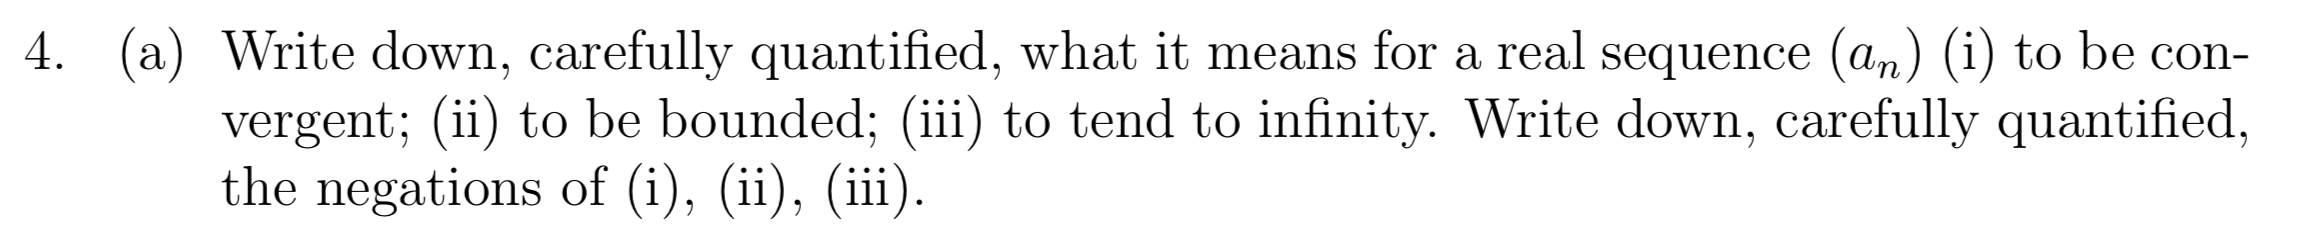
\includegraphics[width=400pt]{img/oxford-M2-analysis-I-3-4-a.png}
  \end{mdframed}
  \begin{definition*}\hspace{0pt}
    \begin{enumerate}[label=(\roman*)]
    \item $(a_n)$ is convergent if there exists $L \in \R$ such that for all $\epsilon > 0$ there
      exists $N \in \N$ such that $|a_n - L| < \epsilon$ for all $n \geq N$:
      \begin{align*}
        \exists L \in \R ~~ \forall \epsilon > 0 ~~ \exists N \in \N ~~ \forall n \geq N ~~ |a_n - L| < \epsilon.
      \end{align*}
      $(a_n)$ is not convergent if for all $L \in \R$ there exists $\epsilon > 0$ such that ``no
      $N$ works'':
      \begin{align*}
        \forall L \in \R ~~ \exists \epsilon > 0 ~~ \forall N \in \N ~~ \exists n \geq N ~~ |a_n - L| \geq \epsilon.
      \end{align*}
    \item $(a_n)$ is bounded if there exists $M \in \R$ such that $|a_n| < M$ for all $n \in \N$:
      \begin{align*}
        \exists M \in \R ~~ \forall n \in \N ~~ |a_n| < M.
      \end{align*}
      $(a_n)$ is not bounded if no $M \in \R$ is a bound:
      \begin{align*}
        \forall M \in \R ~~ \exists n \in \N ~~ |a_n| \geq M.
      \end{align*}
    \item $(a_n)$ tends to infinity if for all $M \in \R$ there exists $N \in \N$ such that $a_n > M$ for
      all $n \geq N$:
      \begin{align*}
        \forall M \in \R ~~ \exists N \in \N ~~ \forall n \geq N ~~ a_n > M.
      \end{align*}
      $(a_n)$ does not tend to infinity if there exists $M \in \R$ such that ``no $N$ works'':
      \begin{align*}
        \exists M \in \R ~~ \forall N \in \N ~~ \exists n \geq N ~~ a_n \leq M.
      \end{align*}
    \end{enumerate}
  \end{definition*}
\item\hspace{0pt}
  \begin{mdframed}
    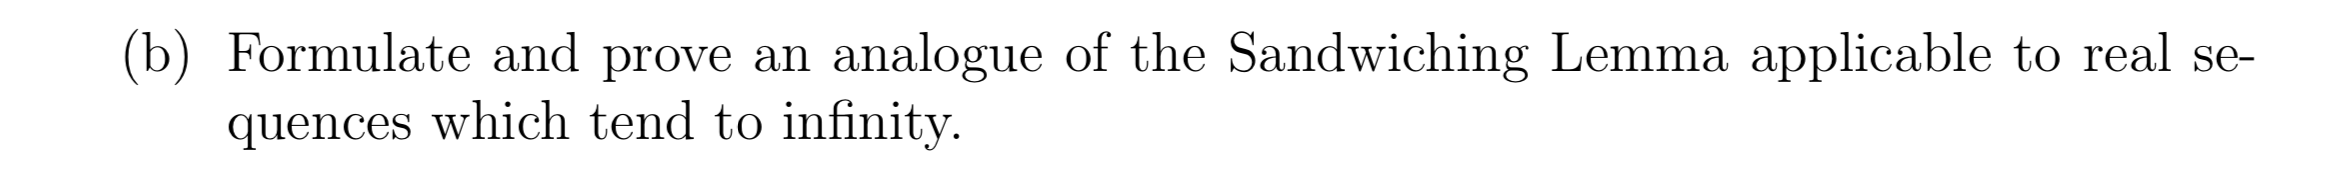
\includegraphics[width=400pt]{img/oxford-M2-analysis-I-3-4-b.png}
  \end{mdframed}
  \begin{theorem*}
    Let $(a_n) \in \R^\N$ and let $(b_n) \in \R^\N$ tend to infinity. If $a_n \geq b_n$ for all
    $n \in \N$ then $a_n$ tends to infinity.
  \end{theorem*}
  \begin{proof}
    Let $(a_n) \in \R^\N$ and let $(b_n) \in \R^\N$ tend to infinity. Suppose $a_n \geq b_n$ for
    all $n \in \N$. Let $M \in \R$ be such that $\exists N \in \N ~~ \forall n \geq N ~~ b_n >
    M$. Then $\forall n \geq N ~~ a_n > M$, therefore $a_n$ tends to infinity.
  \end{proof}
\newpage
\item\hspace{0pt}
  \begin{mdframed}
    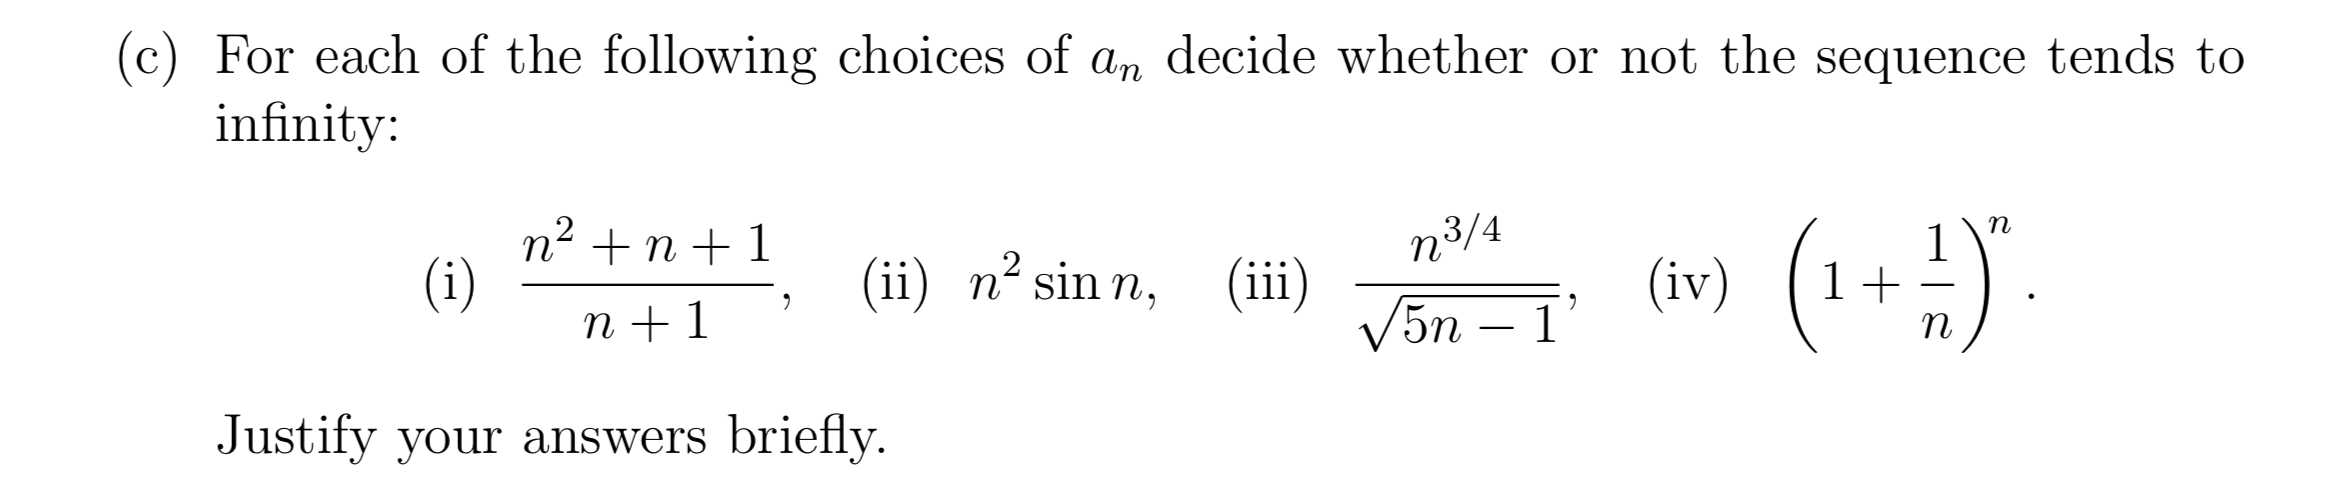
\includegraphics[width=400pt]{img/oxford-M2-analysis-I-3-4-c.png}
  \end{mdframed}
  \begin{enumerate}[label=(\roman*)]
  \item
    \begin{align*}
      \frac{n^2 + n + 1}{n + 1} > \frac{n^2}{n + 1} = \frac{n}{1 + 1/n}.
    \end{align*}
    This tends to infinity \red{TODO: proof}
  \item $n^2\sin n$
  \end{enumerate}
\end{enumerate}

\newpage
\subsection{}
\begin{mdframed}
  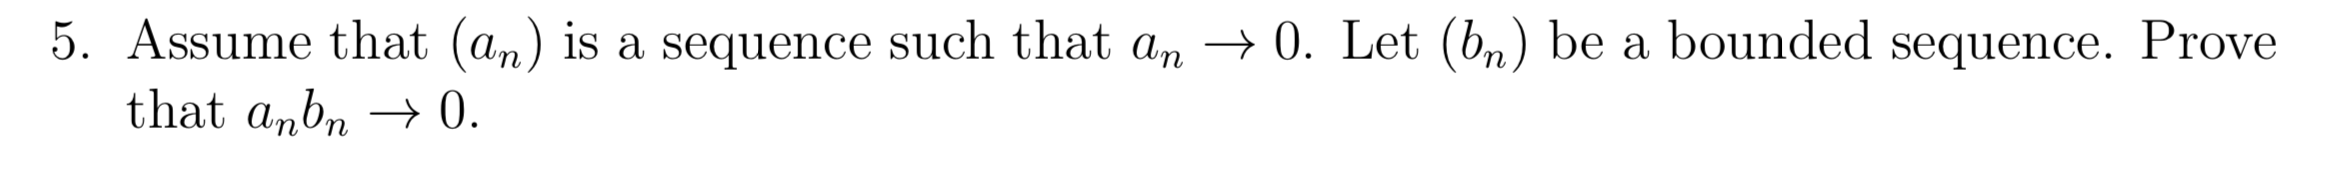
\includegraphics[width=400pt]{img/oxford-M2-analysis-I-3-5-1.png}
\end{mdframed}
\begin{claim*}
  Let $(a^n)$ be a sequence such that $a_n \to 0$. Let $(b_n)$ be a bounded sequence. Then
  $a_nb_n \to 0$.

  % I.e. $(\forall \epsilon > 0) ~~ (\exists N \in \N) ~~ (\forall n \geq N) ~~ (|a_nb_n| < \epsilon)$
\end{claim*}
\begin{proof}
  Let $(a^n)$ be a sequence such that $a_n \to 0$. Let $(b_n)$ be a bounded sequence.

  Let $M$ be a bound for $(b_n)$ so that $|b_n| \leq M$ for all $n$.

  Fix $\epsilon > 0$ and let $N$ be such that $|a_n| < \frac{\epsilon}{M}$ for all $n \geq N$.

  Then $|a_nb_n| = |a_n||b_n| < \epsilon$ for all $n \geq N$.
\end{proof}

\begin{mdframed}
  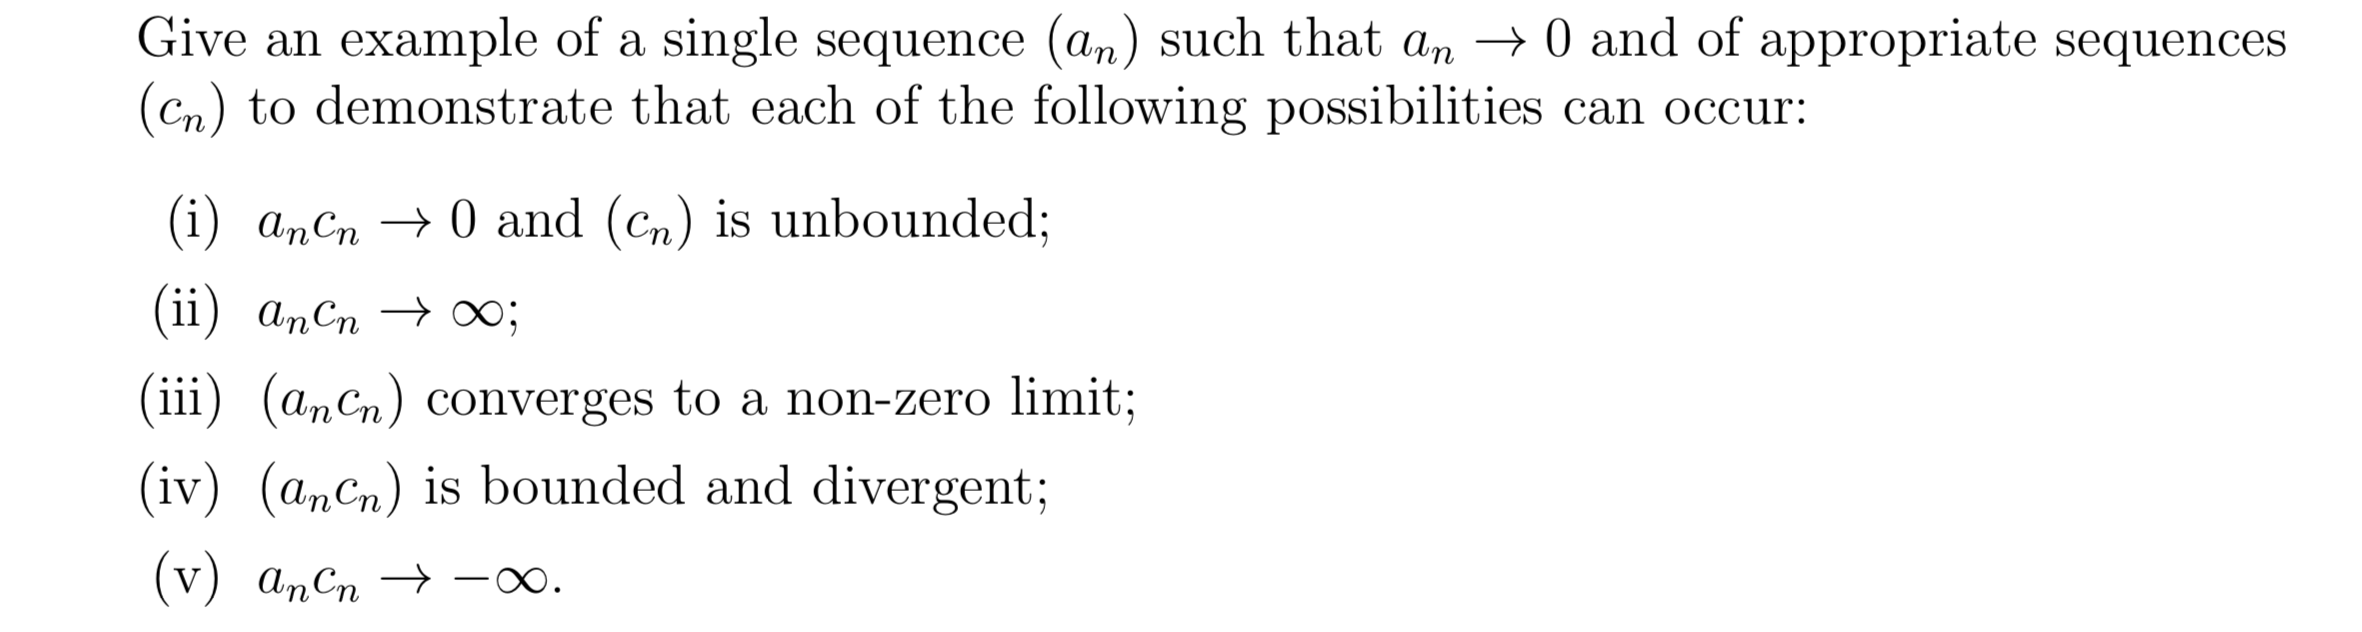
\includegraphics[width=400pt]{img/oxford-M2-analysis-I-3-5-2.png}
\end{mdframed}

\begin{enumerate}[label=(\roman*)]
\item Let $(c_n)$ be unbounded and let $a_n = 0$ for all $n$. Then $a_nc_n \to 0$.
\item Let $c_n = \frac{n}{a_n}$. Then $a_nc_n = n \to \infty$.
\item Let $L \neq 0$ and $c_n = \frac{L}{a_n}$. Then $a_nc_n = L$.
\item Let $c_n = \frac{\sin n}{a_n}$. Then $(a_nc_n) = (\sin n)$ which is bounded and divergent.
\item Let $c_n = \frac{-n}{a_n}$. Then $a_nc_n = n \to -\infty$.
\end{enumerate}

\newpage
\subsection{}
\begin{mdframed}
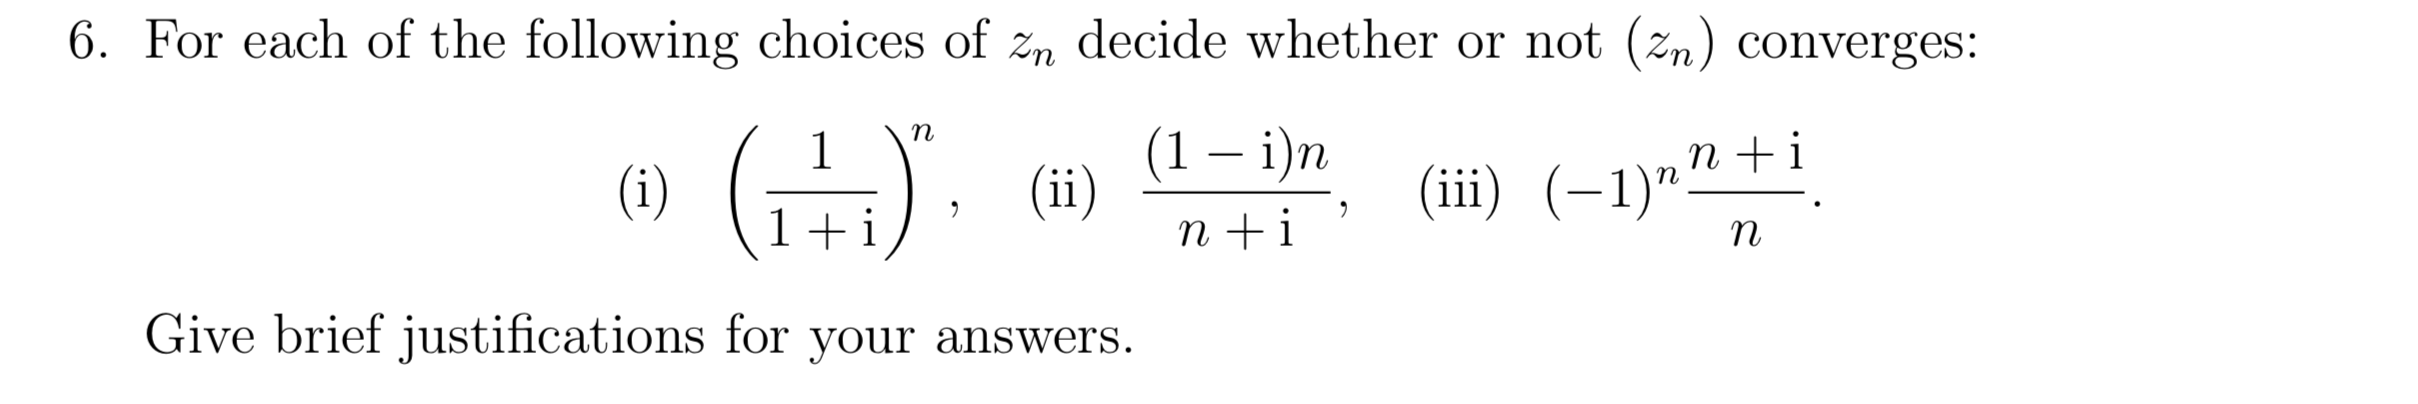
\includegraphics[width=400pt]{img/oxford-M2-analysis-I-3-6.png}
\end{mdframed}

\begin{enumerate}[label=(\roman*)]
\item
\end{enumerate}

\newpage
\subsection{}
\begin{mdframed}
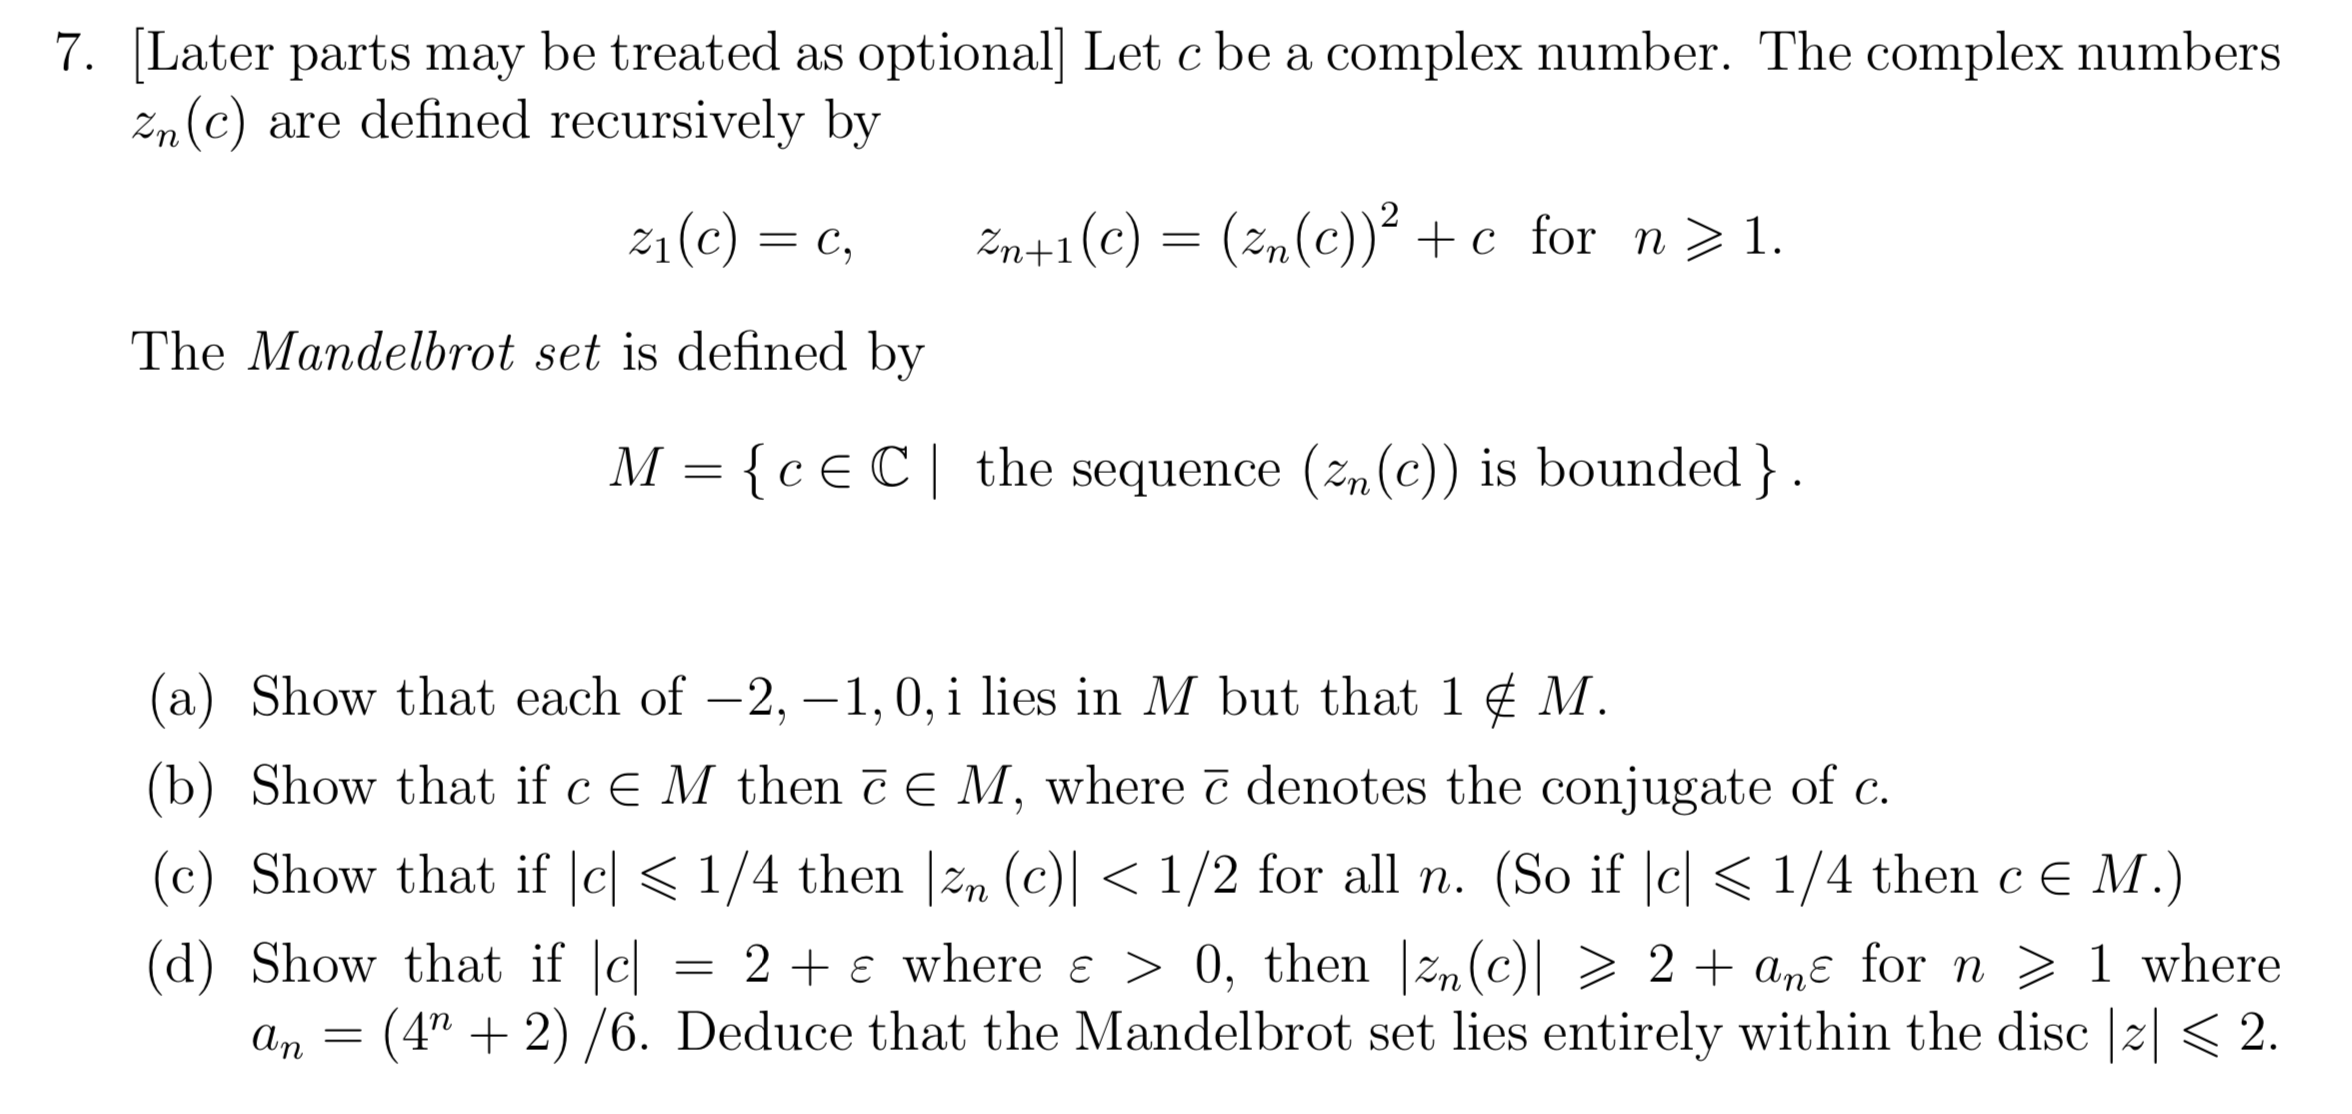
\includegraphics[width=400pt]{img/oxford-M2-analysis-I-3-7.png}
\end{mdframed}



\newpage
\section{Misc}
\newpage
\begin{definition*}[floor and ceil]
  Let $x \in \R$. Then floor of $x$ is $\floor{x} = \max\{n \in \Z ~|~ n \leq x\}$ and ceil of $x$
  is $\ceil{x} = \min\{n \in \Z ~|~ n \geq x\}$.
\end{definition*}

\begin{theorem*}[$\floor{x}$ and $\ceil{x}$ exist]~\\
  Let $x \in \R$. Define $S = \{n \in \Z ~|~ n \geq x\} \subset \R$. Note that $S$ is bounded below
  by $x$. Also $S$ is non-empty by the Archimedean Property of $\N$, since otherwise $x$ would be
  an upper bound for $\N$. Therefore $\ceil{x} = \min S$ exists by Well-Ordering.

  Similarly, $\floor{x}$ exists.
\end{theorem*}

\begin{mdframed}
  (Question from Alex Coward)\\

  Define $f:\R\to\R$ by
  \begin{align*}
    f(x) =
    \begin{cases}
      0 ~~~~~~~~~~  & x \in (\R\setminus\Q)\cup\{0\}\\
     \frac{1}{q}    & x = \frac{p}{q} \in \Q, \gcd(p, q) = 1, q > 0.
    \end{cases}
  \end{align*}
  Where is $f$ continuous?
\end{mdframed}

\begin{definition*}[Stride]
  Let $S = \big\{\frac{1}{q} ~|~ q \in \N\big\}$. For $x = \frac{p}{q} \in \Q$, where
  $\gcd(p, q) = 1$, $q > 0$, define the stride function $s:\Q\to S$ by $x \mapsto \frac{1}{q}$. We
  say that the stride of $x$ is $s(x)$.
\end{definition*}

% \begin{intuition*}
%   At rational $x$, $f(x)$ returns the largest stride that hits $x$ when starting from zero. At
%   irrational $x$ (and zero), $f(x) = 0$.
% \end{intuition*}

\begin{claim*}
  $f$ is continuous at $0$, i.e. $\lim_{x \to 0}f(x) = 0$.
\end{claim*}

\begin{proof}
  Fix $\epsilon > 0$ and take $\delta = \epsilon$. We claim that
  $0 < |x| < \delta \implies |f(x)| < \epsilon$.

  At irrational values $0 < |x| < \delta$, we have $|f(x)| = 0 < \epsilon$.

  At rational values $0 < |x| < \delta$, we have $x = \frac{p}{q} \in \Q, \gcd(p, q) = 1$ for some
  $p \in \Z, q \in \N$ with $p, q \neq 0$. Therefore
  \begin{align*}
    |f(x)| = \Big|\frac{1}{q}\Big| \leq \Big|\frac{p}{q}\Big| = |x| < \delta = \epsilon.
  \end{align*}
\end{proof}

\begin{claim*}
  $f$ is continuous on $\R\setminus\Q$.
\end{claim*}

\begin{proof}
  Let $a \in \R\setminus\Q$ and fix $0 < \epsilon < 1$. Note that $f(a) = 0$. We now construct an
  interval centered at $a$ that excludes rational numbers with stride greater than or equal to
  $\epsilon$.

  Formally, we claim that there exists $\delta > 0$ such that
  $0 < |x - a| < \delta \implies |f(x)| < \epsilon$.

  Define $T = \{\frac{1}{n} ~|~ n \in \N, \frac{1}{n} > \epsilon\}$. Note that $T$ is non-empty
  since $\epsilon < 1$ therefore $1 \in T$. Since $T$ is non-empty, finite, and bounded below,
  $\min T$ exists. Let $\frac{1}{m} = \min T$.

  Let $K = \{k \in \N ~|~ k < m\}$, so that $\frac{1}{k} \geq \epsilon$ for all $k \in K$.

  For each $k \in K$ define $U_k$ by $U_k = \{\frac{n}{k} ~|~ \frac{n}{k} < a, n \in \N\}$. Note
  that $\max U_k$ exists and is equal to $\frac{\floor{ak}}{k}$ (\red{Proof needed?}). Let
  $u^* = \max ~ \{\max U_K ~|~ k \in K\}$.

  Now perform the analogous procedure for values greater than $a$. For each $k \in K$ define $V_k$
  by $V_k = \{\frac{n}{k} ~|~ \frac{n}{k} > a, n \in \N\}$. Note that $\min V_k$ exists and is
  equal to $\frac{\ceil{ak}}{k}$. Let $v^* = \min ~ \{\min V_K ~|~ k \in K\}$.

  Set $\delta = \min(|a - u^*|, |a - v^*|)$. Then
  $0 < |x - a| < \delta \implies |f(x)| < \epsilon$.
\end{proof}

\begin{claim*}
  $f$ is not continuous on $\Q$.
\end{claim*}

\begin{proof}
  Let $a \in \Q\setminus\{0\}$. Then $f(a) = s(a)$, the stride of $a$. Suppose for a contradiction
  that $f$ is continuous at $a$. Let $\epsilon = s(a)/2$. Then there exists $\delta > 0$ such that
  $|x - a| < \delta \implies |f(x) - s(a)| < \epsilon$. Note that there exists
  $b \in (a, a + \delta) \cap \R\setminus\Q$, since there is an irrational number between any two
  real numbers. But $|f(b) - s(a)| = s(a) > \epsilon$, a contradiction. Therefore $f$ is not
  continuous at $a$.
\end{proof}

(I thought I would need the following as a lemma to prove that minima of $U_k$ and $V_k$ above
exist, but I have not used it.)
\begin{theorem*}[well-order isomorphism]
  Let $S$ be a set with a well-ordering. I.e. every non-empty subset of $S$ has a least
  element. Let $T$ be a set and let $f:S \to T$ be a bijection with the property that
  \begin{align*}
    s_1 \leq s_2 \iff f(s_1) \leq f(s_2).
  \end{align*}
  Then $<$ is a well-ordering on $T$.
\end{theorem*}
\begin{proof}
  Let $\emptyset \neq U \subseteq T$. We claim that $\min T$ exists and is given by
  $\min T = f(\min S)$. Indeed suppose that there exists $t \in T$ such that $t < f(\min S)$. But
  then $f^\1(t) < \min S$, a contradiction. Therefore $\min T = f(\min S)$ as claimed.
\end{proof}

\end{document}